%
% Economics & Politics of the Quantum Internet
%

\dropcap{A}{ny} form of computation comes at an economic cost, but also brings with it a payoff. A key consideration in any model for computation is the tradeoff between the two. Because the computational power of quantum computers scales inherently differently than classical computers, we expect economic indicators to exhibit different scaling characteristics and dynamics also, thereby fundamentally altering the economic landscape of the post-quantum world.

We will now treat some of these economic issues in the context of a global network of unified quantum computing resources, which are then equitably time-shared\index{Time-sharing}. We argue in Sec.~\ref{sec:time_share} that this time-shared model for quantum computation is always more computationally efficient than having distinct quantum computers operating independently in parallel, owing to the super-linear scaling in their joint computational power. While this section provides mathematical details of various economic models, Secs.~\ref{sec:economics} \& \ref{sec:quant_coin_essay} provide a popular, high-level discussion surrounding these issues. Sec.~\ref{sec:summary_economic_models} summarises the various economic models we present in this part.

%
% Classical-Equivalent Computational Power & Computational Scaling Functions
%

\section{Classical-equivalent computational power \& computational scaling functions}\index{Classical-equivalent computational power}\index{Computational scaling functions}\label{sec:comp_sc_func}

\dropcap{L}{et} $t$ be the classical-equivalent runtime\index{Classical-equivalent computational power} of a quantum algorithm comprising $n$ qubits -- that is, how long would a given classical computer require to implement this $n$-qubit quantum computation? We define a \textit{computational scaling function}\index{Computational scaling functions} characterising this relationship,

\begin{definition}[Computational scaling functions] \label{def:scaling_func}\index{Computational scaling functions} 
The computational scaling function, $f_\mathrm{sc}$, relates the number of qubits held by a quantum computer, $n$, and the classical-equivalent runtime\index{Classical-equivalent runtime}, $t$, of the algorithm it implements,
\begin{align}
t = f_\mathrm{sc}(n),
\end{align}
	where $f_\mathrm{sc}$ is monotonically increasing, and depends heavily on both the algorithm being implemented, as well as the architecture of the computer, including the computational model and choice of fault-tolerance protocol.
\end{definition}

The exact form of the scaling function will be specific to the algorithm being deployed\footnote{For example, the \textit{circuit depth}\index{Circuit depth}, i.e number of gate applications in series, will heavily influence the number of classical steps required to simulate the circuit.}, and the computational model (e.g cluster states vs the circuit model, as well as choices in error correction, amongst other factors). Most notably, different quantum algorithms offer different scalings in their quantum speedup -- Grover's algorithm (Sec.~\ref{sec:quantum_search})\index{Grover's algorithm} offers only a quadratic quantum speedup, compared to the exponential speedup afforded by Shor's algorithm (Sec.~\ref{sec:shors_alg})\index{Shor's algorithm}. Thus, the computational scaling function depends on both the hardware and software, and may therefore differ between different users operating the same computer. We abstract this away and assume all these factors and resource overheads have been merged into the scaling function.

%
% Virtual Scaling Functions
%

\subsection{Virtual computational scaling functions}\index{Virtual computational scaling functions}

If a network of quantum computers were combined into a single, larger \textit{virtual quantum computer}\index{Virtual quantum computer} (Sec.~\ref{sec:GVQC}) using a distributed model for quantum computation (Sec.~\ref{sec:dist_QC}), we can define a computational scaling function relationship for the virtual device,

\begin{definition}[Virtual scaling function]\index{Virtual computational scaling functions}
The joint classical-equivalent runtime\index{Classical-equivalent computational power} of a distributed virtual quantum computation over a network is,
\begin{align}
t_\mathrm{joint} = f_\mathrm{sc}^\mathrm{virtual}(n_\mathrm{global}),
\end{align}
where,
\begin{align}
n_\mathrm{global} = \sum_{j\in\mathrm{nodes}} n_j,
\end{align}
is the total number of qubits in the network, with $j$ summing over all nodes in the network, each of which holds $n_j$ qubits. $f_\mathrm{sc}^\mathrm{virtual}$ is obtained from $f_\mathrm{sc}$ by factoring in network overheads and inefficiencies. With perfect network efficiency, \mbox{$f_\mathrm{sc}^\mathrm{virtual}=f_\mathrm{sc}$}.
\end{definition}

%
% Combined Computational Scaling Functions
%

\subsection{Combined computational scaling functions}\index{Combined computational scaling functions}\label{sec:comb_comp_sc_func}

Until now we have characterised the entire network by a single scaling function. Of course, the scaling functions observed by different market participants needn't all be the same, as they are functions of not only the hardware, but also the participants' different algorithmic applications (i.e software).

Consider taking a single unit of time (i.e we are ignoring cost discounting\index{Cost discounting} over multiple units of time) and dividing it amongst a number of nodes, $n_\mathrm{nodes}$, each with their own scaling function, $f_\mathrm{sc}^{(i)}$. The total classical-equivalent runtime of the computation is additive, given simply by a linear combination of the classical-equivalent processing times of the individual nodes. This yields the relationship for combining scaling functions,
\begin{definition}[Combined scaling functions]\index{Combined computational scaling functions}\label{def:comb_sc_func}
The effective combined computational scaling function, $f_\mathrm{sc}^\mathrm{(joint)}$, of a group of participants, each with their own scaling functions, $f_\mathrm{sc}^{(i)}$, is given by,
\begin{align}
	t_\mathrm{joint} &= \sum_{i=1}^{n_{\mathrm{nodes}}} \beta_i \cdot f_\mathrm{sc}^{(i)}(n_\mathrm{global}) \nonumber \\
	&= f_\mathrm{sc}^\mathrm{(joint)}(n_\mathrm{global}),
\end{align}
where $\beta_i$ characterise the share of processing time allocated to each node, and for normalisation,
\begin{align}
\sum_{i=1}^{n_\mathrm{nodes}} \beta_i = 1.
\end{align}

\end{definition}

Thus, the joint scaling function of the entire network is simply given by a linear combination (weighted average) of the scaling functions of the different market participants.

%
% Per-qubit computational power
%

\section{Per-qubit computational power}\label{sec:NPSF}\index{Per-qubit computational power}

\dropcap{O}{ne} parameter that appears ubiquitously in the upcoming economic models and warrants a definition of its own is the computational power of a quantum computer per qubit. This relates the power and size of the computer. We define this as the \textit{per-qubit computational power},

\begin{definition}[Per-qubit computational power]\label{def:NPSF}\index{Per-qubit computational power}
The per-qubit computational power is defined as the computational power per qubit,
\begin{align}
\chi_\mathrm{sc}(n) = \frac{f_\mathrm{sc}(n)}{n}.
\end{align}
\end{definition}

This parameter acts as an overall, network size-dependent price scaling factor on:
\begin{itemize}
\item Quantum computational leverage (Sec.~\ref{sec:quant_ec_lev}).
\item Cost of computation (Sec.~\ref{sec:cost_of_comp}).
\item Time-shared computational power (Sec.~\ref{sec:arb_free_time_share}).
\item Quantum computational leverage (Sec.~\ref{sec:quant_ec_lev}).
\item Forward contracts (Sec.~\ref{sec:for_contr}).
\end{itemize}

This parameter lends itself to the elegant interpretation as a cost multiplier on qubit asset, dividend and derivative prices, which warrants investigation of its scaling characteristics, shown in Fig.~\ref{fig:NPSF}. 

Note that in the quantum context, the computational power per qubit is not intrinsic to the qubit itself, but depends on how many qubits it cooperates with, a phenomena which does not arise in the classical context.

The key observation is that this scaling factor is constant for classical computing, where the scaling function is linear, but monotonically increasing for any super-linear scaling function. For polynomial scaling functions, it has the effect of reducing the order of the polynomial by one. And for exponential scaling functions, it remains exponential.

\begin{figure}[htb!]\index{Per-qubit computational power}
	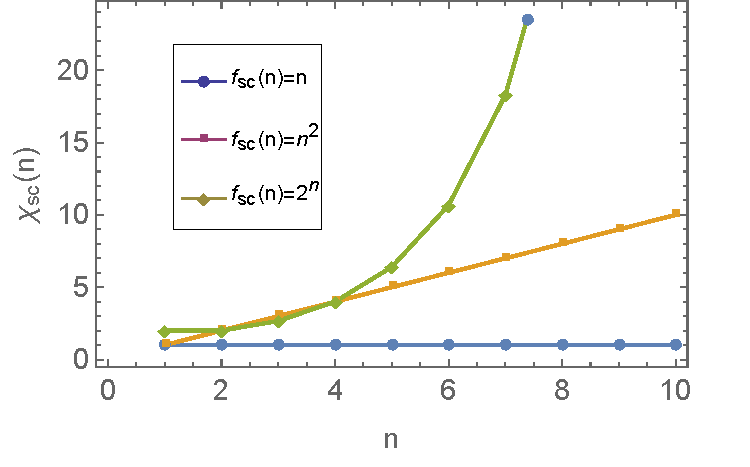
\includegraphics[clip=true, width=0.475\textwidth]{network_price_scaling_factor}
	\captionspacefig \caption{Per-qubit computational power, $\chi_\mathrm{sc}$, as a function of several representative computational scaling functions, $f_\mathrm{sc}$, where $n$ is network size.} \label{fig:NPSF}
\end{figure}

%
% Time-Sharing
%

\section{Time-sharing}\label{sec:time_share}\index{Time-sharing}

\dropcap{S}{uppose} Alice and Bob both possessed expensive classical Cray\texttrademark\,supercomputers\index{Supercomputers}, both identical. They're both connected to the internet, so does it make sense to unify their computational resources over the network to construct a more powerful virtual machine\index{Virtual quantum computer}, which they subsequently time-share\index{Time-sharing} between themselves, or are they better off just using their own computers independently?

If there were an asymmetry in demand for computational resources, it would make perfect sense to unify computational resources, so as to mitigate wasting precious clock-cycles. However, if they were both heavy users, always consuming every last clock-cycle, it would make no difference: for a given computation, Alice and Bob could each be allocated half the processing time of the virtual supercomputer twice as powerful; or, each could exploit the full processing time of their half-as-fast computers. In either case, the dollar cost of the computation is the same. This simple observation follows trivially from the linear relationship between processing power and the number of CPUs in a classical computer.

More generally, in a networked environment where time-sharing\index{Time-sharing} of classical computational resources is applied equitably, proportionate to nodes' contribution to the network, the dollar cost per computation is (roughly, modulo parallelisation overheads) unaffected by the rest of the network. Instead, the motivation for networking computational resources is to improve efficiency by ensuring that clock-cycles are not wasted, but instead distributed according to demand by a scheduling algorithm, which could be market-driven, for example.

However, the computational power of a quantum computer generally doesn't scale linearly with its number of qubits, but super-linearly, often exponentially. This completely changes the economics, and market dynamics of networked quantum computers. Intuitively, we expect equitable time-sharing of unified quantum computational resources to offer more performance to all nodes than if they were to exclusively use their own resources in isolation. That is, the cost of a computation is reduced by resource-sharing, even after time-sharing.

For this reason, henceforth we will assume an environment in which owners of quantum hardware network and unify their computational power, sharing the virtual quantum computer's power between them.

In Sec.~\ref{sec:arb_free_time_share} we present an explicit model for equitable time-sharing, which is optimal from a market perspective.

%
% Economic Model Assumptions
%

\section{Economic model assumptions}

\dropcap{B}{efore} proceeding with explicit derivations of economic models, we state some assumptions about the dynamics of a marketplace in quantum assets. These assumptions are largely based on historical observations surrounding classical technologies that we might reasonably expect to also apply in the quantum era. However, given that the quantum marketplace is one that hasn't been explored in detail until now, it may be the case that some of these assumptions will require revision. Nonetheless, the general techniques we employ could readily be adapted to some relaxations and variations in these assumptions.

%
% Efficient Markets
%

\subsection{Efficient markets}\label{sec:eff_markets} \index{Efficient markets}

We make several assumptions about the efficiency of the quantum marketplace. These are largely based on the conventional efficient-market hypothesis (EMH)\index{Efficient-market hypothesis (EMH)} \cite{???}, readily taught in undergraduate ECON101 and subsequently summarily rejected upon entering ECON202. For ease of exposition, we will remain in the ECON101 classroom.

Some of these assumptions may reasonably turn out to be invalid, or require revision as we learn more about upcoming quantum technologies and the trajectories their marketplace will follow. However, for ease of exposition, and the purposes of presenting some initial rudimentary, \textit{qualitative} analyses and thought experiments, these assumptions simplify our derivations and act as a good starting point for future, more rigorous treatment (which we highly encourage!).

Given that the quantum marketplace doesn't actually exist yet, it isn't immediately clear which assumptions are likely to be valid or not, and future, more sophisticated models will inevitably need to make more appropriate assumptions. Certainly it's no secret that in conventional settings the EMH is flawed in many respects, and some of its idealised assumptions break down in reality.

\begin{postulate}[Efficient markets]\label{post:market_eff}\index{Efficient markets} We make the following efficiency assumptions on the dynamics of the quantum marketplace:
\begin{itemize}
	\item Qubits are a `scarce' resource --- there is always positive, non-zero demand for them.\index{Scarcity}
	\item No wastage --- quantum computational resources are always fully utilised, with no down-time.\index{Wastage}
	\item Transaction free --- transaction costs are negligible, for both quantum assets and their derivatives.\index{Transaction cost}
	\item Negligible cost-of-carry --- e.g storage and maintenance costs are negligible.\index{Cost of carry}
	\item High liquidity --- it is always possible to execute transactions at market rates.\index{Liquidity}
	\item Perfect competition --- there are no monopolies gouging prices, which are in equilibrium.\index{Perfect competition}
	\item Arbitrage-free --- market rates for different assets and derivatives are perfectly consistent, with no opportunity for `free money' by trading on market discrepancies.\index{Arbitrage-free}
	\item Perfect information --- all market participants have complete knowledge of all market variables, including one another.\index{Perfect information}
	\item Rational markets --- all market participants act rationally\footnote{i.e with perfect economic self-interest \latinquote{Avaritia}.} upon available information.\index{Rational markets}
	\item Indefinite asset lifetime --- there is no deterioration or death of quantum hardware over time.\index{Asset lifetime}
	\item There is a risk-free rate of return ($r_\mathrm{rf}$)\index{Risk-free rate of return}
-- the rate of growth exhibited by an investment into an optimal risk-free asset\footnote{Historically these risk-free assets are taken as being US government bonds\index{US government bonds}\index{Risk-free asset}, with the bond yield being the risk-free RoR.}
	\end{itemize}
\end{postulate}

%
% Central Mediating Authority
%

\subsection{Central mediating authority}\index{Central mediating authority}

In Sec.~\ref{sec:time_share} we argued that because of the super-linear scaling in the computational power of networked quantum computers, it will be most economically efficient to unify the world's entire collective quantum computational resources over the network and time-share their joint computational power. For this reason, we will assume that global quantum computing resources are unified, and time-shared equitably (as will be described in Sec.~\ref{sec:arb_free_time_share}), overseen by a trusted central authority, congruent with our efficient market assumptions (Sec.~\ref{sec:eff_markets}).

The role of the mediating authority is to perform process scheduling\index{Scheduling} -- equitably allocating algorithmic runtime on the virtual computer to the different network participants. This could be in the form of a state-backed authority, or open market-driven alliances. In any case, the job of the authority is a relatively straightforward one, and we will assume it induces negligible cost and computational overhead, remaining largely transparent to the end-user.

However, as discussed in Sec.~\ref{sec:GVQC}, it may be the case that competing strategic interests will drive a wedge between the quantum resources of competitors and adversaries, partitioning them into a set of smaller networks, divided across strategic boundaries. In this instance, the arguments presented in the upcoming sections will apply to these smaller, isolated networks individually.

%
% Network Growth
%

\subsection{Network growth} \index{Network!Growth}

We assume the number of qubits in the global network in the future is growing exponentially over time, i.e the rate of progress of quantum technology will observe a Moore's Law-like behaviour, as with the classical transistor.

This is a reasonable assumption based on the observation of this ubiquitous kind of behaviour in present-day technologies. Classical computing has been on a consistent exponential trajectory since the 1980's, and although it must eventually asymptote, it shows no sign of doing so in the immediate future. Quantum technologies sit at the entry point to this trajectory, and we expect it to continue for the medium-term. Thus, we let the number of qubits in the network be,
\begin{postulate}[Network growth]\label{post:net_growth}\index{Network!Growth}
The number of qubits in the global quantum internet is growing exponentially over time as,
\begin{align}
	N(t) = N_0 {\gamma_N}^{t},
\end{align}
where \mbox{$\gamma_N\geq 1$} characterises the rate of exponential growth in the number of qubits available to the quantum network.
\end{postulate}

The exact value of the growth rate, $\gamma_N$, is obviously unclear at such early stages in the development of the market and will ultimately be determined empirically. Although in the case of classical computing we have seen a very consistent doubling of computational power roughly every 18 months. This may very well be different for quantum technologies, owing to their fundamentally different engineering requirements (which are far more challenging in general).

%
% Hardware Cost
%

\subsection{Hardware cost} \index{Hardware cost}

Let the dollar cost of physical qubits follow Moore's Law-like dynamics, decreasing exponentially with time,
\begin{postulate}[Hardware cost]\label{post:hardware_cost}\index{Hardware cost}
The dollar-cost of a single physical qubit scales inverse exponentially against time as,
\begin{align}
	C(t) = C_0 {\gamma_C}^{-t},
\end{align}
where \mbox{$\gamma_C\geq 1$} characterises the decay rate.
\end{postulate}

This is consistent with the observed evolution of classical hardware since the beginning of the digital revolution, and it is reasonable to think that technological progress in the quantum era will follow a similar trajectory.

%
% Network Power
%

\section{Network power}\index{Network!Power}\label{sec:network_power}

\dropcap{F}{irst} and foremost, with a fully interconnected quantum computational network, what is the projection of its net computational power now and into the future? This is simply obtained via the joint computational scaling function applied to projected network size,

\begin{postulate}[Network power]\label{post:network_power}\index{Network!Power}
The combined computational power of the entire network, measured in classical-equivalent runtime (i.e FLOPs), is given by,
\begin{align}
P(t) &= f_\mathrm{sc}(n_\mathrm{global})\nonumber \\
&= f_\mathrm{sc}(N_0{\gamma_N}^t).
\end{align}
\end{postulate}

%
% Network Value
%

\section{Network value}\index{Network!Value}\label{sec:network_value}

\dropcap{T}{he} simplest economic metric one might define is the collective dollar value of the entire network. That is, the product of the number of qubits on the network and the dollar cost per physical qubit at a given time.

\begin{postulate}[Network value]\label{post:network_value}\index{Network!Value}
The dollar-value of the entire network is given by,
\begin{align}
	V(t) &= C(t) N(t) \nonumber \\
	&= C_0 N_0 \left(\frac{\gamma_N}{\gamma_C}\right)^t.
\end{align}
\end{postulate}

Note that the collective value of the network appreciates exponentially if the rate of network growth is greater than the rate of decay in the value of physical qubits, otherwise it depreciates. At \mbox{$\gamma_C=\gamma_N$} the network's dollar value remains constant over time, even if it continues expanding. This is shown in Fig.~\ref{fig:network_value}.

\begin{figure}[!htbp]
	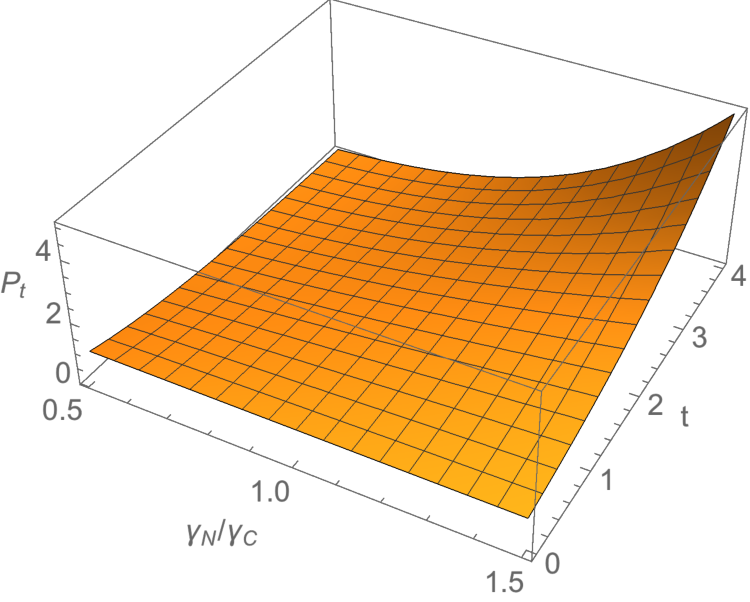
\includegraphics[clip=true, width=0.4\textwidth]{network_value}
	\captionspacefig \caption{Dollar value (in units of \mbox{$C_0N_0$}) of the network as a function of time, growth rate in the number of physical qubits, and rate of decay in the dollar value of physical qubits. When \mbox{$\gamma_N/\gamma_C=1$} the network's value remains constant over time. Above this the network's value appreciates exponentially, and below which it depreciates exponentially against time.} \label{fig:network_value}
\end{figure}

%
% Rate of Return
%

\section{Rate of return}\index{Rate of return}

\dropcap{T}{he} execution of computations typically has monetary value to the consumer. After all, they are paying hard-earned money for access to the technology!

Suppose the owners of the quantum hardware are not running computations themselves, but rather are collectively licensing out their joint compute-time to end-users. The hardware owners will of course be demanding a profit from their enterprise. The rate at which they earn back their investment into hardware via the licensing of compute-time, we will refer to as the rate of return (RoR), $\gamma_\mathrm{ror}$. We define this as,

\begin{postulate}[Rate of return]\label{post:RoR}\index{Rate of return}
The RoR is defined as,
\begin{align}
e^{\gamma_\mathrm{ror}} = \frac{n_\mathrm{return}}{n_\mathrm{cost}},
\end{align}
where $n_\mathrm{return}$ is the profit made by licensing out the network's joint compute-power for a single unit of time, given a present-day network value of $n_\mathrm{cost}$.
\end{postulate}

A higher $\gamma_\mathrm{ror}$ implies a faster payback rate on hardware investment\footnote{We have parameterised the RoR as an exponential for convenience when performing derivations with compounding.}.

In an ideal market, where hardware cost is completely predictable, e.g perfectly follows the hardware cost model (Pos.~\ref{post:hardware_cost}), the risk asymptotes to zero and perfect arbitrage (Pos.~\ref{post:market_eff}) will drive the RoR to asymptote to the risk-free RoR, \mbox{$\gamma_\mathrm{ror} \to r_\mathrm{rf}$}. Of course, real markets necessarily exhibit risks and uncertainties, and the RoR on quantum hardware will never be truly risk-free, meaning that upon trading off risk for return, we will always observe \mbox{$\gamma_\mathrm{ror} > r_\mathrm{rf}$}.

%
% Cost Of Computation
%

\section{Cost of computation}\label{sec:cost_of_comp} \index{Cost of computation}

\dropcap{I}{n} the same scenario as before, where compute-time is being licensed out to end-users, the hardware owners return over a single unit of time equates to the cost of computation over that period.

Let $L(t)$ be the dollar-value of utilising the network's computing resources for a single unit of time. This is obtained as the return made on the value of the network per FLOP,
\begin{postulate}[Cost of computation]\label{post:cost_comp}
The efficient-market dollar-value of a computation for a single unit of time at time $t$, per FLOP is,
\begin{align}\index{Cost of computation}
	L(t) &= \frac{e^{\gamma_\mathrm{ror}} P(t)}{V(t)} \nonumber\\
	&= \frac{e^{\gamma_\mathrm{ror}} C_0{\gamma_C}^{-t}}{\chi_\mathrm{sc}(N_0 {\gamma_N}^t)},
\end{align}
\end{postulate}
which implies,
\begin{postulate}[Spot price of computation]\index{Spot price of computation} The present-day (\mbox{$t=0$}) spot price of a computation per FLOP is,
\begin{align}
L(0) = \frac{e^{\gamma_\mathrm{ror}}C_0}{\chi_\mathrm{sc}(N_0)}.	
\end{align}
\end{postulate}
That is, the value of computations simply approximates the return on initial hardware investment, scaled by its initial computational power, as is intuitively expected.

Note that if $f_\mathrm{sc}$ scales linearly, as per classical computation, we observe a regular exponential decay in the cost of computation, consistent with the classical Moore's Law. On the opposing extreme, for exponentially quantum-enhanced $f_\mathrm{sc}$, the cost of computation decreases super-exponentially with time, an economic behaviour unique to post-classical computation with no classical analogue.

The time-derivative of the cost of computation is strictly negative, assuming correctness of the growth and cost postulates (Pos.~\ref{post:net_growth} \& \ref{post:cost_comp}),
\begin{align}
\frac{\partial L}{\partial t} \leq 0,	
\end{align}
which implies monotonic reduction in the cost of computation over time, unless network growth and cost completely freeze (\mbox{$\gamma_N=\gamma_C=0$}), in which case the cost of computation remains flat.

Examples of the temporal dynamics of the cost of computation are shown in Fig.~\ref{fig:econ_cost_of_comp} for representative computational scaling functions.

\if 2\pubmode
\begin{figure}[!htbp]
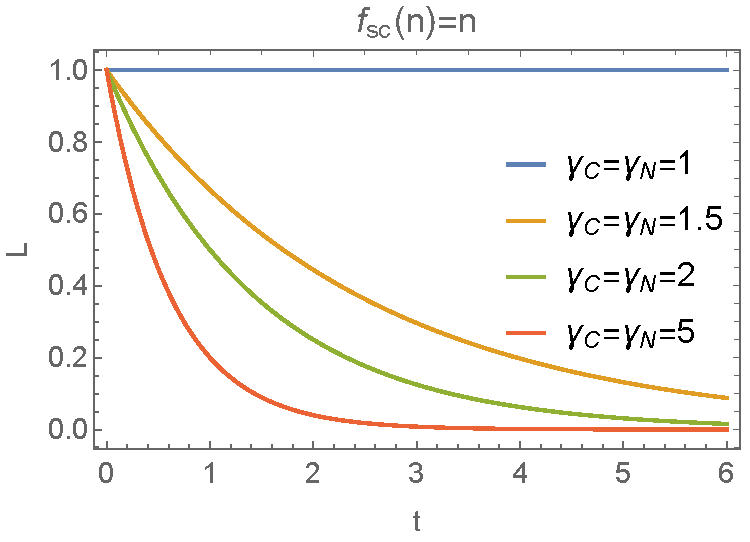
\includegraphics[clip=true, width=0.4\textwidth]{cost_of_comp_n}\\
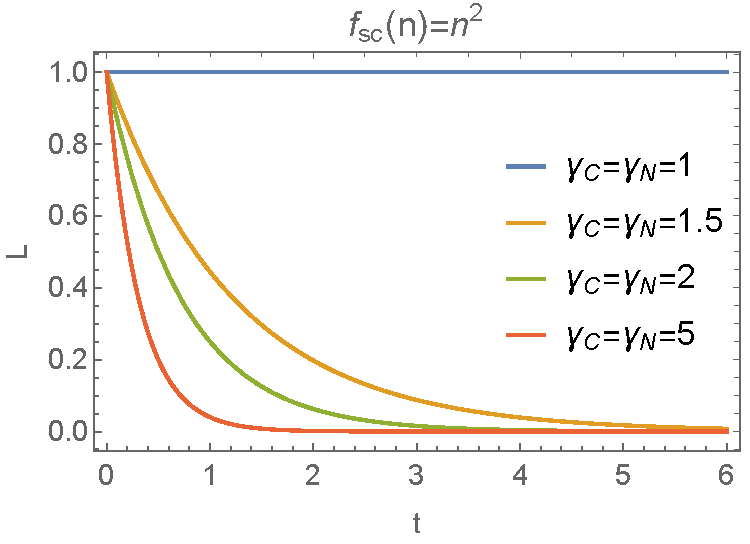
\includegraphics[clip=true, width=0.4\textwidth]{cost_of_comp_n2}\\
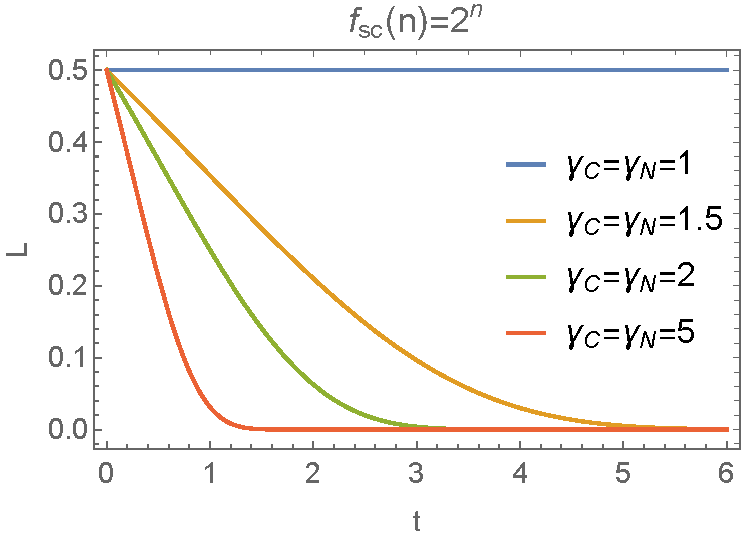
\includegraphics[clip=true, width=0.4\textwidth]{cost_of_comp_2n}
\captionspacefig \caption{Examples of the temporal dynamics of the cost of computation for different scaling functions and exponential growth rates. Units are \mbox{$C_0=N_0=n=1$}, with RoR \mbox{$\gamma_\mathrm{ror}=0$}. A non-zero RoR would simply scale these figures by a constant factor of $e^{\gamma_\mathrm{ror}}$.}\label{fig:econ_cost_of_comp}
\end{figure}
\else
\begin{figure*}[!htbp]
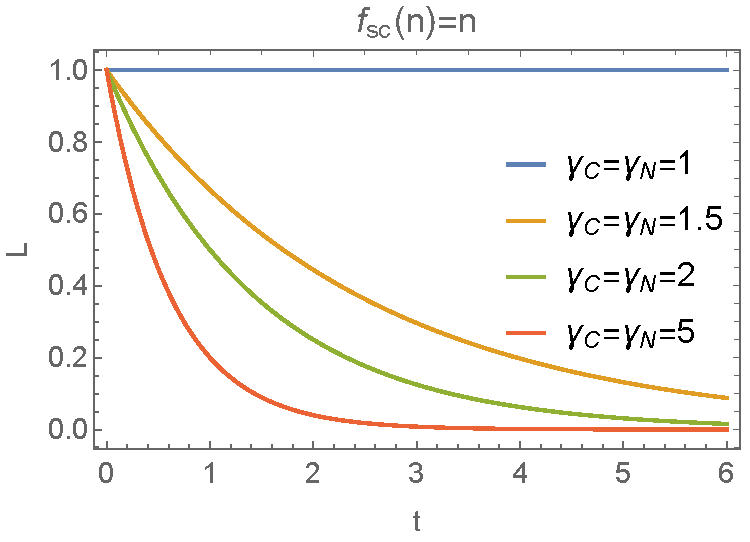
\includegraphics[clip=true, width=0.325\textwidth]{cost_of_comp_n}
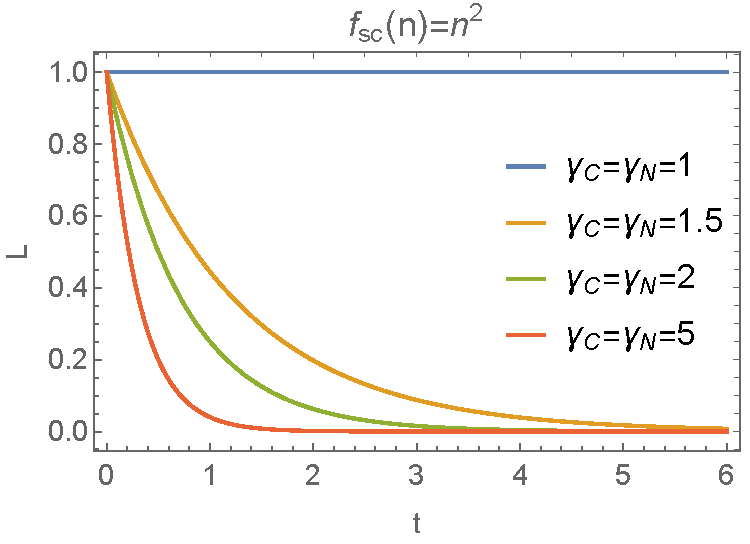
\includegraphics[clip=true, width=0.325\textwidth]{cost_of_comp_n2}
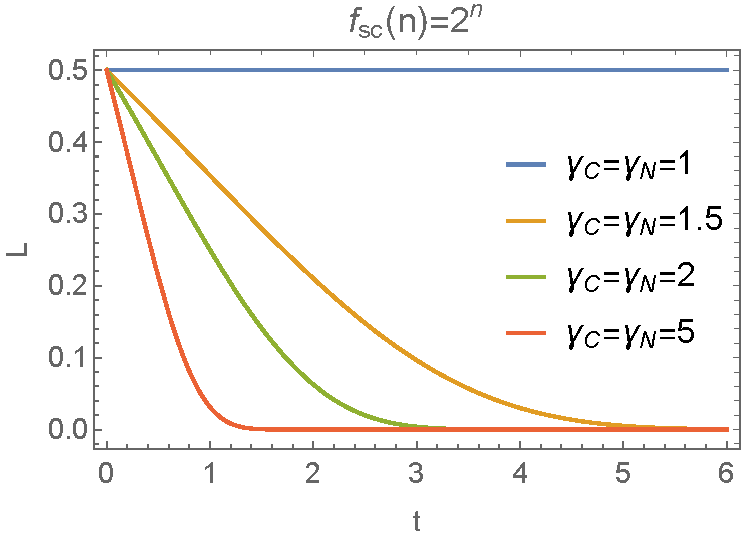
\includegraphics[clip=true, width=0.325\textwidth]{cost_of_comp_2n}
\captionspacefig \caption{Examples of the temporal dynamics of the cost of computation for different scaling functions and exponential growth rates. Units are \mbox{$C_0=N_0=n=1$}, with RoR \mbox{$\gamma_\mathrm{ror}=0$}. A non-zero RoR would simply scale these figures by a constant factor of $e^{\gamma_\mathrm{ror}}$.}\label{fig:econ_cost_of_comp}
\end{figure*}
\fi

%
% Arbitrage-Free Time-Sharing
%

\section{Arbitrage-free time-sharing model}\label{sec:arb_free_time_share} \index{Arbitrage-free time-sharing model}\index{Time-sharing}

\dropcap{I}{n} the context of our time-shared global network of unified quantum computers (Sec.~\ref{sec:time_share}), how do we fairly and equitably allocate time-shares between contributors? We now derive an elementary arbitrage-free model for equitable time-sharing in such a network.

Let,
\begin{align}
	0\leq r_n \leq 1,
\end{align}
be the proportion of compute-time allocated to a node in possession of $n$ qubits, in a global network of $n_\mathrm{global}$ qubits. Arbitrage in the value of physical qubits will enforce the linearity constraint,
\begin{align}
	r_{n_1+n_2} = r_{n_1} + r_{n_2}.
\end{align}
This constraint effectively mandates that `all qubits are created equal', and two qubits are twice as valuable as one \latinquote{Qubit aequalitatem}. Were, for example, a bundle of two qubits more expensive than two individual qubits purchased in isolation, a market participant could perform arbitrage and unfairly gain free compute-time by buying two qubits separately, unifying them, selling the bundle, buying them back individually, and repeating indefinitely until he seizes the entire network.

Additionally, we have assumed no compute-cycles are wasted -- compute-time is always fully utilised, as per Pos.~\ref{post:market_eff}. Then it follows that the time-share of the combined resources of the entire network should be unity,
\begin{align}
	r_{n_\mathrm{global}}=1.
\end{align}
\mbox{$r_{n_\mathrm{global}}<1$} would imply inefficiency via wasted clock-cycles. Combining this with the linearity constraint implies the arbitrage-free time-sharing model,
\begin{definition}[Arbitrage-free time-sharing model] \label{def:arb_free_ts}\index{Arbitrage-free time-sharing model}
In an efficient market for unified quantum computing time-shares\index{Time-sharing}, a network participant in possession of $n$ of the entire $n_\mathrm{global}$ qubits in the network is entitled to the fraction of unified network compute time,
\begin{align}\index{Time-shared compute-time}
	r_n = \frac{n}{n_\mathrm{global}},
\end{align}
where,
\begin{align}
n_\mathrm{global} = \sum_{j\in\mathrm{nodes}} n_j,
\end{align}
is the total number of qubits in the network, and,
\begin{align}
0\leq r_n \leq 1.	
\end{align}
\mbox{$r_n=1$} iff the node has a complete monopoly over qubits, i.e \mbox{$n=n_\mathrm{global}$}.
\end{definition}

Based on this equitable model for time-sharing,
\begin{definition}[Time-shared computing power]\index{Time-shared computing power}
The computing power allocated to each user under the arbitrage-free time-sharing model is,
\begin{align}
	c_n &= r_n \cdot f_\mathrm{sc}(n_\mathrm{global}) \nonumber \\
	&= n \cdot \chi_\mathrm{sc}(n_\mathrm{global}).
\end{align}
\end{definition}

This model is intuitively unsurprising, since it is analogous to the case of classical computer clusters -- nodes receive a time-share proportional to the proportion of the hardware they are contributing to the network. However, it is important to point out that the arbitrage is taking place in the cost of physical qubits, but not in terms of the dollar value of their classical-equivalent processing power, since this is in general non-linearly related to the number of qubits. Arbitrage in computational power per se is complicated by the fact that it is a non-fungible asset that cannot be directly traded, or uniquely associated with a tangible, tradable asset -- its computational value is a function of other assets.

%
% Problem Size Scaling Functions
%

\section{Problem size scaling functions}\index{Problem size!Scaling functions}\label{sec:prob_sc_func}

\dropcap{T}{he} computational scaling function\index{Computational scaling functions} introduced previously expresses the power of a quantum computer in terms of its classical-equivalent runtime, or equivalently FLOPs\index{FLOPs}. However, this may not be the metric of interest when considering a computer's algorithmic power. In many situations, of far greater interest is the size of a problem\index{Problem size} instance that can be solved in a given timespan. For example, the FLOPs associated with solving an instance of a 3-\textsc{SAT} problem\index{3-SAT problem} grows exponentially with the number of clauses. When discussing the execution of this problem on a given computer, what we really want to know is how many clauses our device can cope with, rather than what the classical-equivalent runtime is.

This observation motivates us to re-parameterise the power of quantum computers in terms of the problem size of a given algorithm to be solved. Employing the same methodology as for computational scaling functions, we define the \textit{problem size scaling function}, which relates the size of an algorithmic problem to it's classical equivalent runtime. Then equating the computational and problem size scaling function yields,

\begin{definition}[Problem size scaling function]\index{Problem size!Scaling functions}
The problem size scaling function relates the size of a problem instance ($s$), in some arbitrary metric, to its classical-equivalent runtime ($t$) under a time-shared network model,
\begin{align}
t = f_\mathrm{size}(s).
\end{align}
Equating this with the time-shared computational power yields,
\begin{align}
	n\cdot \chi_\mathrm{sc}(n_\mathrm{global}) = f_\mathrm{size}(s).
\end{align}
Isolating the problem size yields,
\begin{align}
s = f_\mathrm{size}^{-1}(n\cdot \chi_\mathrm{sc}(n_\mathrm{global})).
\end{align}
\end{definition}

We now consider several choices of scaling functions.

First let us consider the classical case of linear scaling functions (for both the computational and problem size scaling functions),
\begin{align}
	f_\mathrm{sc}(n) &= \alpha_\mathrm{sc} n,\nonumber\\
	f_\mathrm{size}(s) &= \alpha_\mathrm{size} s.
\end{align}
Solving for the problem size simply yields,
\begin{align}
s &= \frac{n}{\alpha_\mathrm{size}} \nonumber\\
&= O(1),
\end{align}
where $n$ is regarded as a constant, and $n_\mathrm{global}$ is a variable parameter of the network. That is, the problem sizes of solvable instances is independent of the size of the external network with whom we are time-sharing. This is to be expected, since these scaling functions are typical of classical computers.

For polynomial scaling functions,
\begin{align}
f_\mathrm{sc}(n) &= n^{p_\mathrm{sc}},\nonumber\\
f_\mathrm{size}(s) &= s^{p_\mathrm{size}}.
\end{align}
This yields problem size,
\begin{align}
	s &= (n \cdot {n_\mathrm{global}}^{p_\mathrm{sc}-1})^\frac{1}{p_\mathrm{size}} \nonumber\\
	&= O(\mathrm{poly}(n_\mathrm{global})),
\end{align}
demonstrating polynomial scaling in our solvable problem size against the size of the network.

For exponential scaling functions,
\begin{align}
f_\mathrm{sc}(n) &= e^{\alpha_\mathrm{sc}n},\nonumber\\
f_\mathrm{size}(s) &= e^{\alpha_\mathrm{size}s},
\end{align}
we obtain,
\begin{align}
s &= \log\left(n \frac{e^{\alpha_\mathrm{sc}n_\mathrm{global}}}{\alpha_\mathrm{sc}n_\mathrm{global}}\right) \nonumber\\
&= \alpha_\mathrm{sc}n_\mathrm{global} + \log(n)-\log(\alpha_\mathrm{sc}n_\mathrm{global}) \nonumber\\
&= O(n_\mathrm{global}),
\end{align}
demonstrating that the solvable problem size grows linearly with network size. That is to say, waiting for a doubling in the external network's size will also double the size of a \textbf{BQP}-complete\index{BQP} problem that can be solved in the same time.

%
% Quantum Computational Leverage
%

\section{Quantum computational leverage}\label{sec:quant_ec_lev}\index{Quantum computational leverage}

\dropcap{I}{n} Secs.~\ref{sec:dist_QC} \& \ref{sec:module} we introduced distributed and modularised quantum computation. Using this as a toy model, we will now investigate the market dynamics of uniting the quantum computational resources of multiple market participants, as per an equitable time-sharing model (Sec.~\ref{sec:time_share}). We envisage a model whereby network participants are contributing modules to the networked quantum computer, thereby unifying their computational power.

The $i$th node is contributing the fraction of the hardware $r_i$, and receives this same proportion of compute-time under the arbitrage-free time-sharing model (Def.~\ref{def:arb_free_ts}). This discounts his classical-equivalent processing time\index{Classical-equivalent computational power} to,
\begin{align}
\tau_i = t_\mathrm{joint} \cdot r_i.
\end{align}

We are now interested in quantifying how much better off individual contributors are under this model than they were individually. Let us define the \textit{quantum computational leverage}\index{Quantum computational leverage} (QCL) of a node's quantum computer to be the ratio between their unified time-shared and individual classical-equivalent processing times\index{Classical-equivalent computational power},
\begin{align}
\lambda_i = \frac{\tau_i}{t_i},
\end{align}
yielding the QCL formula,

\begin{definition}[Quantum computational leverage] \label{def:quant_econ_lev}\index{Quantum computational leverage!Formula}\index{Single-qubit quantum computational leverage}
For the $i$th node, and with scaling function $f_{sc}$, the QCL is defined as the ratio between the unified time-shared and individual classical-equivalent algorithmic runtimes,
\begin{align}
\lambda_i &= \frac{\tau_i}{t_i} \nonumber \\
&= \frac{n_i}{n_\mathrm{global}} \cdot \frac{f_{sc}(n_\mathrm{global})}{f_{sc}(n_i)}, \nonumber \\
&= \frac{\chi_\mathrm{sc}(n_\mathrm{global})}{\chi_\mathrm{sc}(n_i)},\nonumber\\
\lambda_i^\mathrm{dB} &= 10\log_{10}(\lambda_i),
\end{align}
where,
\begin{align}
	n_\mathrm{global} = \sum_{j\in \mathrm{nodes}} n_j,
\end{align}
is the total number of qubits in the network. The logarithmic version of the representation in decibels is simply a convenience when dealing with exponential scaling functions.
\end{definition}

Effectively, the QCL tells us how much additional computational power we `get for frbee' by consolidating with the network.

It is extremely important to note that the QCL is asymmetric, in the sense that the leverage achieved by a given node is larger than the leverage achieved by the network, upon the user joining the network (assuming the remainder of the network comprises more qubits than the respective user).

More generally, smaller users achieve higher computational leverage from their investment into quantum hardware than larger users. Specifically,
\begin{align}
	\lambda_i<\lambda_j \,\,\mathrm{for}\,\,n_i>n_j.
\end{align}

For any super-linear scaling function we have \mbox{$\lambda_i > 1 \,\,\forall \, i$}, and for any linear scaling function we have \mbox{$\lambda_i = 1 \,\,\forall \, i$},
\begin{align}
	\lambda=1\,\,\forall\,\,f_\mathrm{sc}(n)=O(n), \nonumber \\
	\lambda>1\,\,\forall\,\,f_\mathrm{sc}(n)>O(n).	
\end{align}

For \mbox{$\lambda_i>1$} it is always computationally beneficial to all nodes to unify computational resources and time-share them equitably, as per the arbitrage-free time-sharing model. Similarly, the distributed network is better off accepting them into the network, albeit to a lesser extent for a large network.

This is in contrast to classical networks, where \mbox{$\lambda\approx 1$}, for any number of nodes in the network (i.e there is no leverage), and it makes no difference whether nodes unify resources or operate independently.

Finally, in the pathological case, where \mbox{$\lambda_i<1$}, nodes are better off working in isolation, a situation which would only naturally arise as a result of algorithmic inefficiencies in parallelisation or distribution.

\begin{definition}[Single-qubit QCL]\index{Single-qubit quantum computational leverage}
The single-qubit QCL is the leverage associated with adding a single qubit to the network, \mbox{$n=1$}, defined as,
\begin{align}
	\lambda_\mathrm{qubit} &= \frac{\chi_\mathrm{sc}(n_\mathrm{global})}{\chi_\mathrm{sc}(1)},\nonumber\\
	\lambda_\mathrm{qubit}^\mathrm{dB} &= 10\log_{10}(\lambda_\mathrm{qubit}).
\end{align}
\end{definition}

Using our postulate for network growth (Pos.~\ref{post:net_growth}) yields the postulated time-dependent QCL,
\begin{postulate}[Time-dependent QCL]
The time-dependent QCL, based on the postulate of exponential network growth, is,
\begin{align}\index{Time-dependent quantum computational leverage}
\lambda_n(t) &= \frac{\chi_\mathrm{sc}(N_0{\gamma_N}^t)}{\chi_\mathrm{sc}(n)},\nonumber\\
\lambda_n^\mathrm{dB}(t) &= 10\log_{10}(\lambda_n(t)),
\end{align}
The initial (\mbox{$t=0$}) time-dependent QCL reduces to the standard QCL formula.
\end{postulate}
Note that for any super-linear scaling function, the time-dependent QCL grows exponentially over time, unlike the classical case where there is no leverage, which does not change over time (i.e \mbox{$\lambda_n(t)=1\,\,\forall\,n,t$}).

The leverage is not merely a function of the hardware, but also of the software applications running upon it, each of which associated with a unique scaling function. Furthermore, it is to be reasonably anticipated that the size of the quantum internet will increase monotonically over time, yielding ever increasing leverage on the initial hardware investment by network contributors.

Examples of the temporal dynamics of the time-dependent single-qubit QCL are shown in Fig.~\ref{fig:time_dep_QCL}.

\begin{figure}[!htbp]
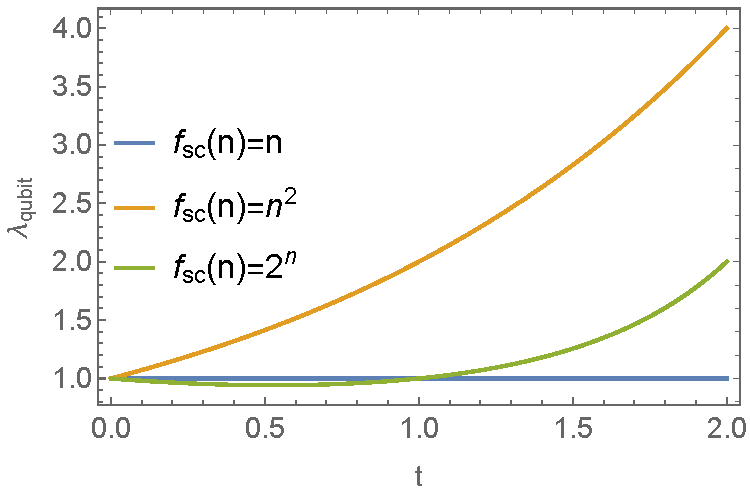
\includegraphics[clip=true, width=0.475\textwidth]{single_qubit_QCL}
\captionspacefig \caption{Time-dependent quantum computational leverage for a single qubit (\mbox{$n=1$}) with different computational scaling functions, under the assumption of exponential network growth in units of \mbox{$N_0=1$}.}\label{fig:time_dep_QCL}
\end{figure}

%
% Static Computational Return
%

\section{Static computational return}\index{Static computational return}\label{sec:static_comp_ret}

\dropcap{T}{he} computational leverage phenomena clearly implies that as the global quantum network expands over time, so too does the computational payback on investment into network expansion, or equivalently, the cost per unit of additional classical-equivalent processing time decreases.

Since exisiting network participants receive leverage upon \textit{other} participants joining the network, an investment into contributing modules has monotonically increasing computational return over time as the network expands, even if that participant ceases making further investment into the network. This is in contrast to classical networks, whereby the computational return upon an investment is fixed over time.

To formalise this, consider the case where a user purchases an initial $n$ qubits, while the global network expands over time as $N_t$. Then the classical-equivalent computational power of the user's fixed investment is,

\begin{definition}[Static computational return]\index{Static computational return} The static computational return is the classical-equivalent processing power of a user's time-share proportion (\mbox{$n/N_t$}), where the user has a fixed investment of $n$ qubits, whereas the network is allowed to expand over time arbitrarily as $N_t$ (e.g according to a quantum Moore's Law),
\begin{align}
	r_\mathrm{static}(t) &= \frac{n\cdot f_\mathrm{sc}(N_t)}{N_t}\nonumber\\
	&= n\cdot\chi_\mathrm{sc}(N_t),
\end{align}
which intuitively follows as the computational power per qubit\index{Per-qubit computational power} in the network, times the number of qubits in our possession.
\end{definition}

Graphical examples for this relationship are equivalent to those presented earlier in Fig.~\ref{fig:NPSF}. In particular, for linear classical scaling functions the return is constant, whereas for exponential quantum scaling functions the return is exponential in network size.

%
% Forward Contract Pricing Model
%

\section{Forward contract pricing model}\label{sec:for_contr}\index{Forward contract pricing model}

\dropcap{F}{orward} contracts are immensely useful in conventional markets, as a means by which to secure future use or ownership of an asset at predictable points in time. For example, farmers make heavy use of forward contracts to lock in sale of their produce before it has been harvested, such that the value is locked in in advance and the sale guaranteed, providing a very valuable hedging instrument\index{Hedging} for managing risk\index{Risk management}.

We envisage similar utility in the context of quantum computing. A company engaging in heavy use of computing power might have a need to perform certain computations at predictable points in the future. In this instance, forward contracts could be very helpful in reducing exposure to risk and guaranteeing access to the technology when needed, at a pre-agreed rate.

Now let us price forward contracts on units of computation, whereby we wish to pay today for the future use of a block of runtime on the global network.

The key observation is that a unit of computation (FLOP) does not carry over time. It must be utilised immediately and cannot be stored for future use. This simplifies the forward price of a unit of computation to simply be the future spot price, discounted by the risk-free RoR, yielding the forward contract pricing model for quantum computing time-shares,
\begin{definition}[Forward contract pricing model] \label{def:forward_cont}\index{Forward contract pricing model}
The efficient market price for a forward contract in a unit of network runtime at future time $T$ is,
\begin{align}
F(T) &= e^{-r_\mathrm{rf}T} L(T)\nonumber\\
&=\frac{e^{\gamma_\mathrm{ror}-r_\mathrm{rf}T} C_0{\gamma_C}^{-T}}{\chi_\mathrm{sc}(N_0 {\gamma_N}^T)}
\end{align}
\end{definition}

Note that in the limit of \mbox{$T\to 0$} this reduces to the spot price of the asset,
\begin{align}
	F(0)=L(0),
\end{align}
as expected.

\if 2\pubmode
\begin{figure}[!htbp]
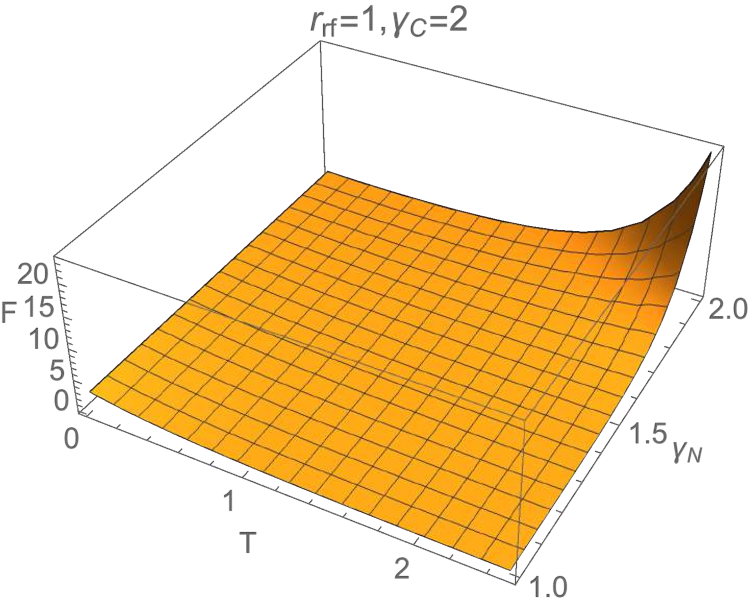
\includegraphics[clip=true, width=0.4\textwidth]{forward_cont_pricing_mod_1}\\
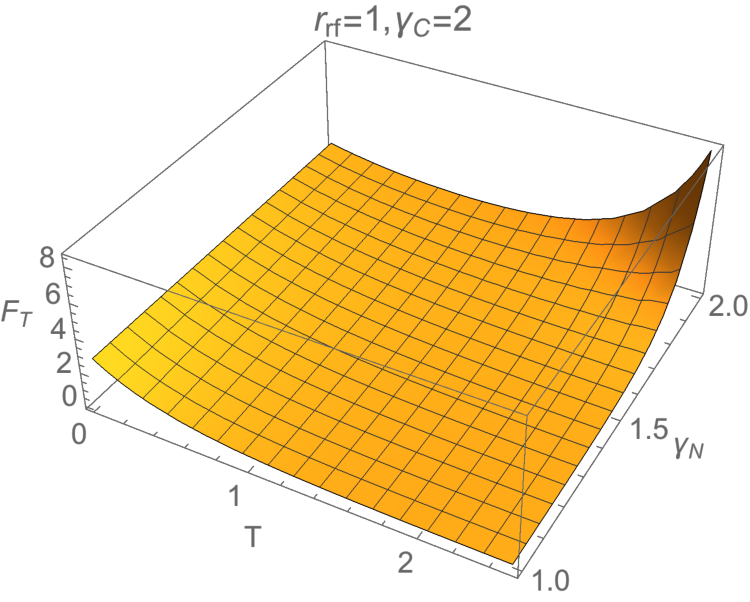
\includegraphics[clip=true, width=0.4\textwidth]{forward_cont_pricing_mod_2}
\captionspacefig \caption{Forward price on a computation to be delivered at time $T$ in the future, in units \mbox{$C_0=N_0=1$}, where we are assuming an exponential scaling function, \mbox{$f_\mathrm{sc}(n)=e^n$}.}\label{fig:forward_cont_pricing_mod}
\end{figure}
\else
\begin{figure*}[!htbp]
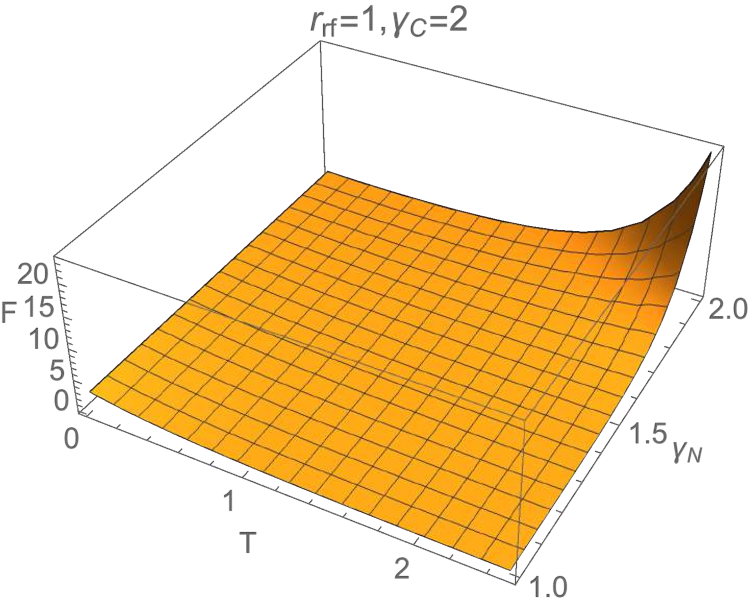
\includegraphics[clip=true, width=0.475\textwidth]{forward_cont_pricing_mod_1}
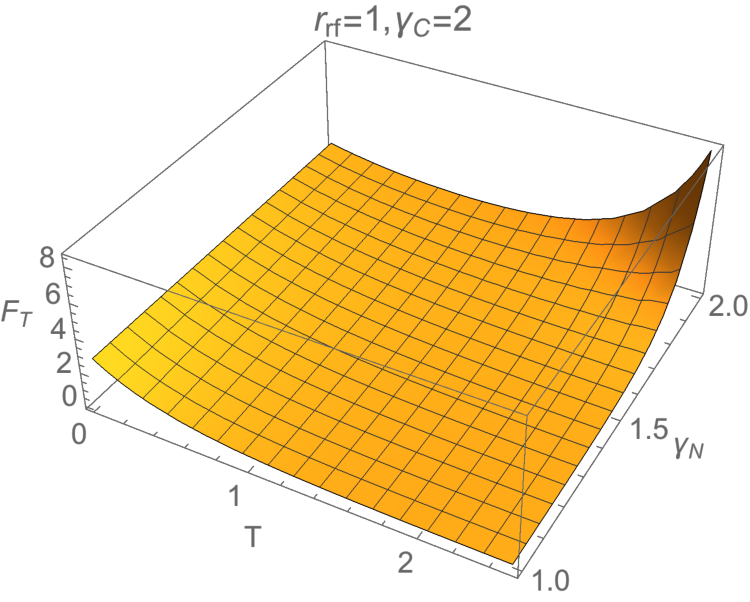
\includegraphics[clip=true, width=0.475\textwidth]{forward_cont_pricing_mod_2}
\captionspacefig \caption{Forward price on a computation to be delivered at time $T$ in the future, in units \mbox{$C_0=N_0=1$}, where we are assuming an exponential scaling function, \mbox{$f_\mathrm{sc}(n)=e^n$}.}\label{fig:forward_cont_pricing_mod}
\end{figure*}
\fi

%
% Political Leverage
%

\section{Political leverage}\index{Political leverage}\label{sec:political_lev}

\dropcap{T}{he} asymmetry in computational leverage observed by parties of different sizes -- specifically, that parties possessing a smaller number of qubits observe greater leverage than those possessing a larger number of qubits -- inevitably will bring with it some power politics, with potentially interesting geo-political implications.

This asymmetry implies that in a globally unified network, were a large party to expel a small party from the network, it would be far more devastating to the computational power of the small party than the larger one. This suggests that inclusion in the global network could be a powerful tool of diplomacy\index{Diplomacy} in the quantum era, where threats of expulsion or resistance to inclusion is the modern day era of gunboat diplomacy\index{Gunboat diplomacy}.

To quantify this we introduce the \textit{political leverage} quantity -- the ratio between the computational leverages observed by two parties belonging to the same network. This directly quantifies the power asymmetry between them.

\begin{definition}[Political leverage]\index{Political leverage}
The political leverage is the ratio between the computational leverages of two parties residing on the same shared network,
\begin{align}
	\gamma_{A,B} &= \frac{\lambda_A}{\lambda_B}\nonumber\\
	&= \frac{\chi_\mathrm{sc}(n_B)}{\chi_\mathrm{sc}(n_A)},\nonumber\\
	\gamma_{A,B}^\mathrm{dB} &= 10\log_{10}(\gamma_{A,B}).
\end{align}
We have the trivial identity that the leverage of $A$ against $B$ is the inverse of the leverage of $B$ against $A$,
\begin{align}
	\gamma_{A,B} &= {\gamma_{B,A}}^{-1},\nonumber\\
	\gamma_{A,B}^\mathrm{dB} &= -\gamma_{B,A}^\mathrm{dB}.
\end{align}
\end{definition}
Note that when two parties are of equal size, there is no power asymmetry and \mbox{$\gamma_{A,B}=1$}. Otherwise, when $A$ and $B$ are unequal, then \mbox{$\gamma_{A,B}\neq 1$}, indicative of power asymmetry. With linear (classical) scaling functions, the political leverage is always unity, \mbox{$\gamma_{A,B}=1$}, regardless of any size asymmetry, whereas for super-linear scaling functions the political leverage diverges.

To the Machiavellian\index{Machiavelli} reader, this quantity can be thought of as answering the question `If I were to expel a party from the network, how much more would it hurt them than it would hurt me?'.

%
% QuantCoin - A Quantum Computation-Backed Cryptocurrency
%

\section{QuantCoin\texttrademark\,-- A quantum computation-backed cryptocurrency}\label{sec:quant_coin_technical}

\dropcap{A}{s} discussed in Sec.~\ref{sec:bitcoin_blockchain}, the Bitcoin\index{Bitcoin} mining\index{Bitcoin!Mining} process involves finding bit-strings that hash\index{Hash!Functions} under SHA256\index{SHA256} to a value within some relatively small range. This so-called `proof-of-work'\index{Proof-of-work} principle associates computational complexity with the mining process, and since the hashing functions are one-way functions, they must be evaluated via brute-force trial-and-error to find hits.

However, what a waste this is! Our proof-of-work is nothing more than hashing a huge number of random bit-strings, computations which are of no intrinsic value to anyone. The market value in turn has nothing to do with any inherent value earned during the mining process. Rather it is based purely on the psychology of scarcity\index{Scarcity}, since there is an upper bound on the number of Bitcoins that satisfy the legitimacy constraint.

What if we were to replace brute-force hashing of random data with computations of genuine monetary value? Then we would have a sounder currency, whose value derives from the monetary cost of executing useful computations. While it is not so easy to invent such a protocol for classical computation, the idea lends itself very naturally to quantum computation, owing to their ability to undergo encrypted computation\index{Encrypted quantum computation} and be subject to verification protocols\index{Verification!Protocols}.

Building upon some of the pricing models introduced earlier in this section, there are two main candidates for backing a cryptocurrency with quantum compute-time:
\begin{itemize}
	\item Spot market\index{Spot market}: we execute the computation immediately in exchange for a coin.
	\item Futures market\index{Futures market}: we own the right to utilise the computer at some fixed time in the future in exchange for a coin.
\end{itemize}
We consider the merits of both these candidates.

A popular-level essay on the future of quantum cryptocurrencies is presented in Sec.~\ref{sec:quant_coin_essay}.

%
% Spot Market Model
%

\subsection{Spot market model}\index{Spot market}

In Alg.~\ref{alg:quant_coin} we provide a very rough sketch for how a protocol based on the spot market might be constructed. A corresponding graphical flowchart is shown in Fig.~\ref{fig:quantcoin_protocol}. We present the ideas in a very high-level manner, abstracting away the physical implementation details of the computation, encryption, and verification protocols, instead envisaging that we can interface with them using a very high-level API\index{API}.

\begin{table}[!htbp]
\begin{mdframed}[innertopmargin=3pt, innerbottommargin=3pt, nobreak]
\texttt{
function QuantCoin($\hat{U}_\mathrm{comp}$, blockchain, data, reward):
\begin{enumerate}
	\item Alice homomorphically/blindly encrypts $data$,
		\begin{align}
			encryptedInput = homoEncrypt(data)
		\end{align}
	\item Alice commits the $encryptedInput$ to the public $blockchain$,
	\begin{align}
	blockchain.commit(encryptedInput)	
	\end{align}
	\item Alice places into escrow Bob's $reward$,
	\begin{align}
		escrow.hold(reward)
	\end{align}
	\item Bob processes the $encryptedInput$,	\begin{align}
		encryptedOutput = \hat{U}_\mathrm{comp}(encryptedInput)
	\end{align}
	\item Bob commits encrypted output to the $blockchain$,
	\begin{align}
	blockchain.commit(encryptedOutput)	
	\end{align}
	\item Alice and Bob execute a verification protocol,
	\begin{align}
	proof = verify(encryptedOutput)	
	\end{align}
	\item The $proof$ is committed to the $blockchain$ (as is every step of the proof if it is an interactive one),
	\begin{align}
		blockchain.commit(proof)
	\end{align}
	\item The $blockchain$ network inspects that the verification is valid.
	\item If valid, the $blockchain$ hashes and signs the data and proof, encapsulating it into a QuantCoin\texttrademark\,token, which is given to Bob,
	\begin{align}
		&token = \mathrm{SHA256}(encryptedInput\nonumber\\
		&+ encryptedOutput + proof)\nonumber\\
		&token.sign(blockchain)\nonumber\\
		&Bob.receive(token)
	\end{align}
	\item The $reward$ held in escrow is released to Bob,
	\begin{align}
		escrow.release(Bob)
	\end{align}
	\item $\Box$
\end{enumerate}}
\end{mdframed}
\captionspacealg \caption{Sketch for how a quantum computation-backed cryptocurrency might be implemented. We have abstracted away the underlying Blockchain protocol, interfacing with it using a high-level API, since Blockchain technology is highly liable to evolve. We similarly call upon verification subroutines using a high-level implementation-independent API.} \label{alg:quant_coin}
\end{table}

\begin{figure}[!htbp]
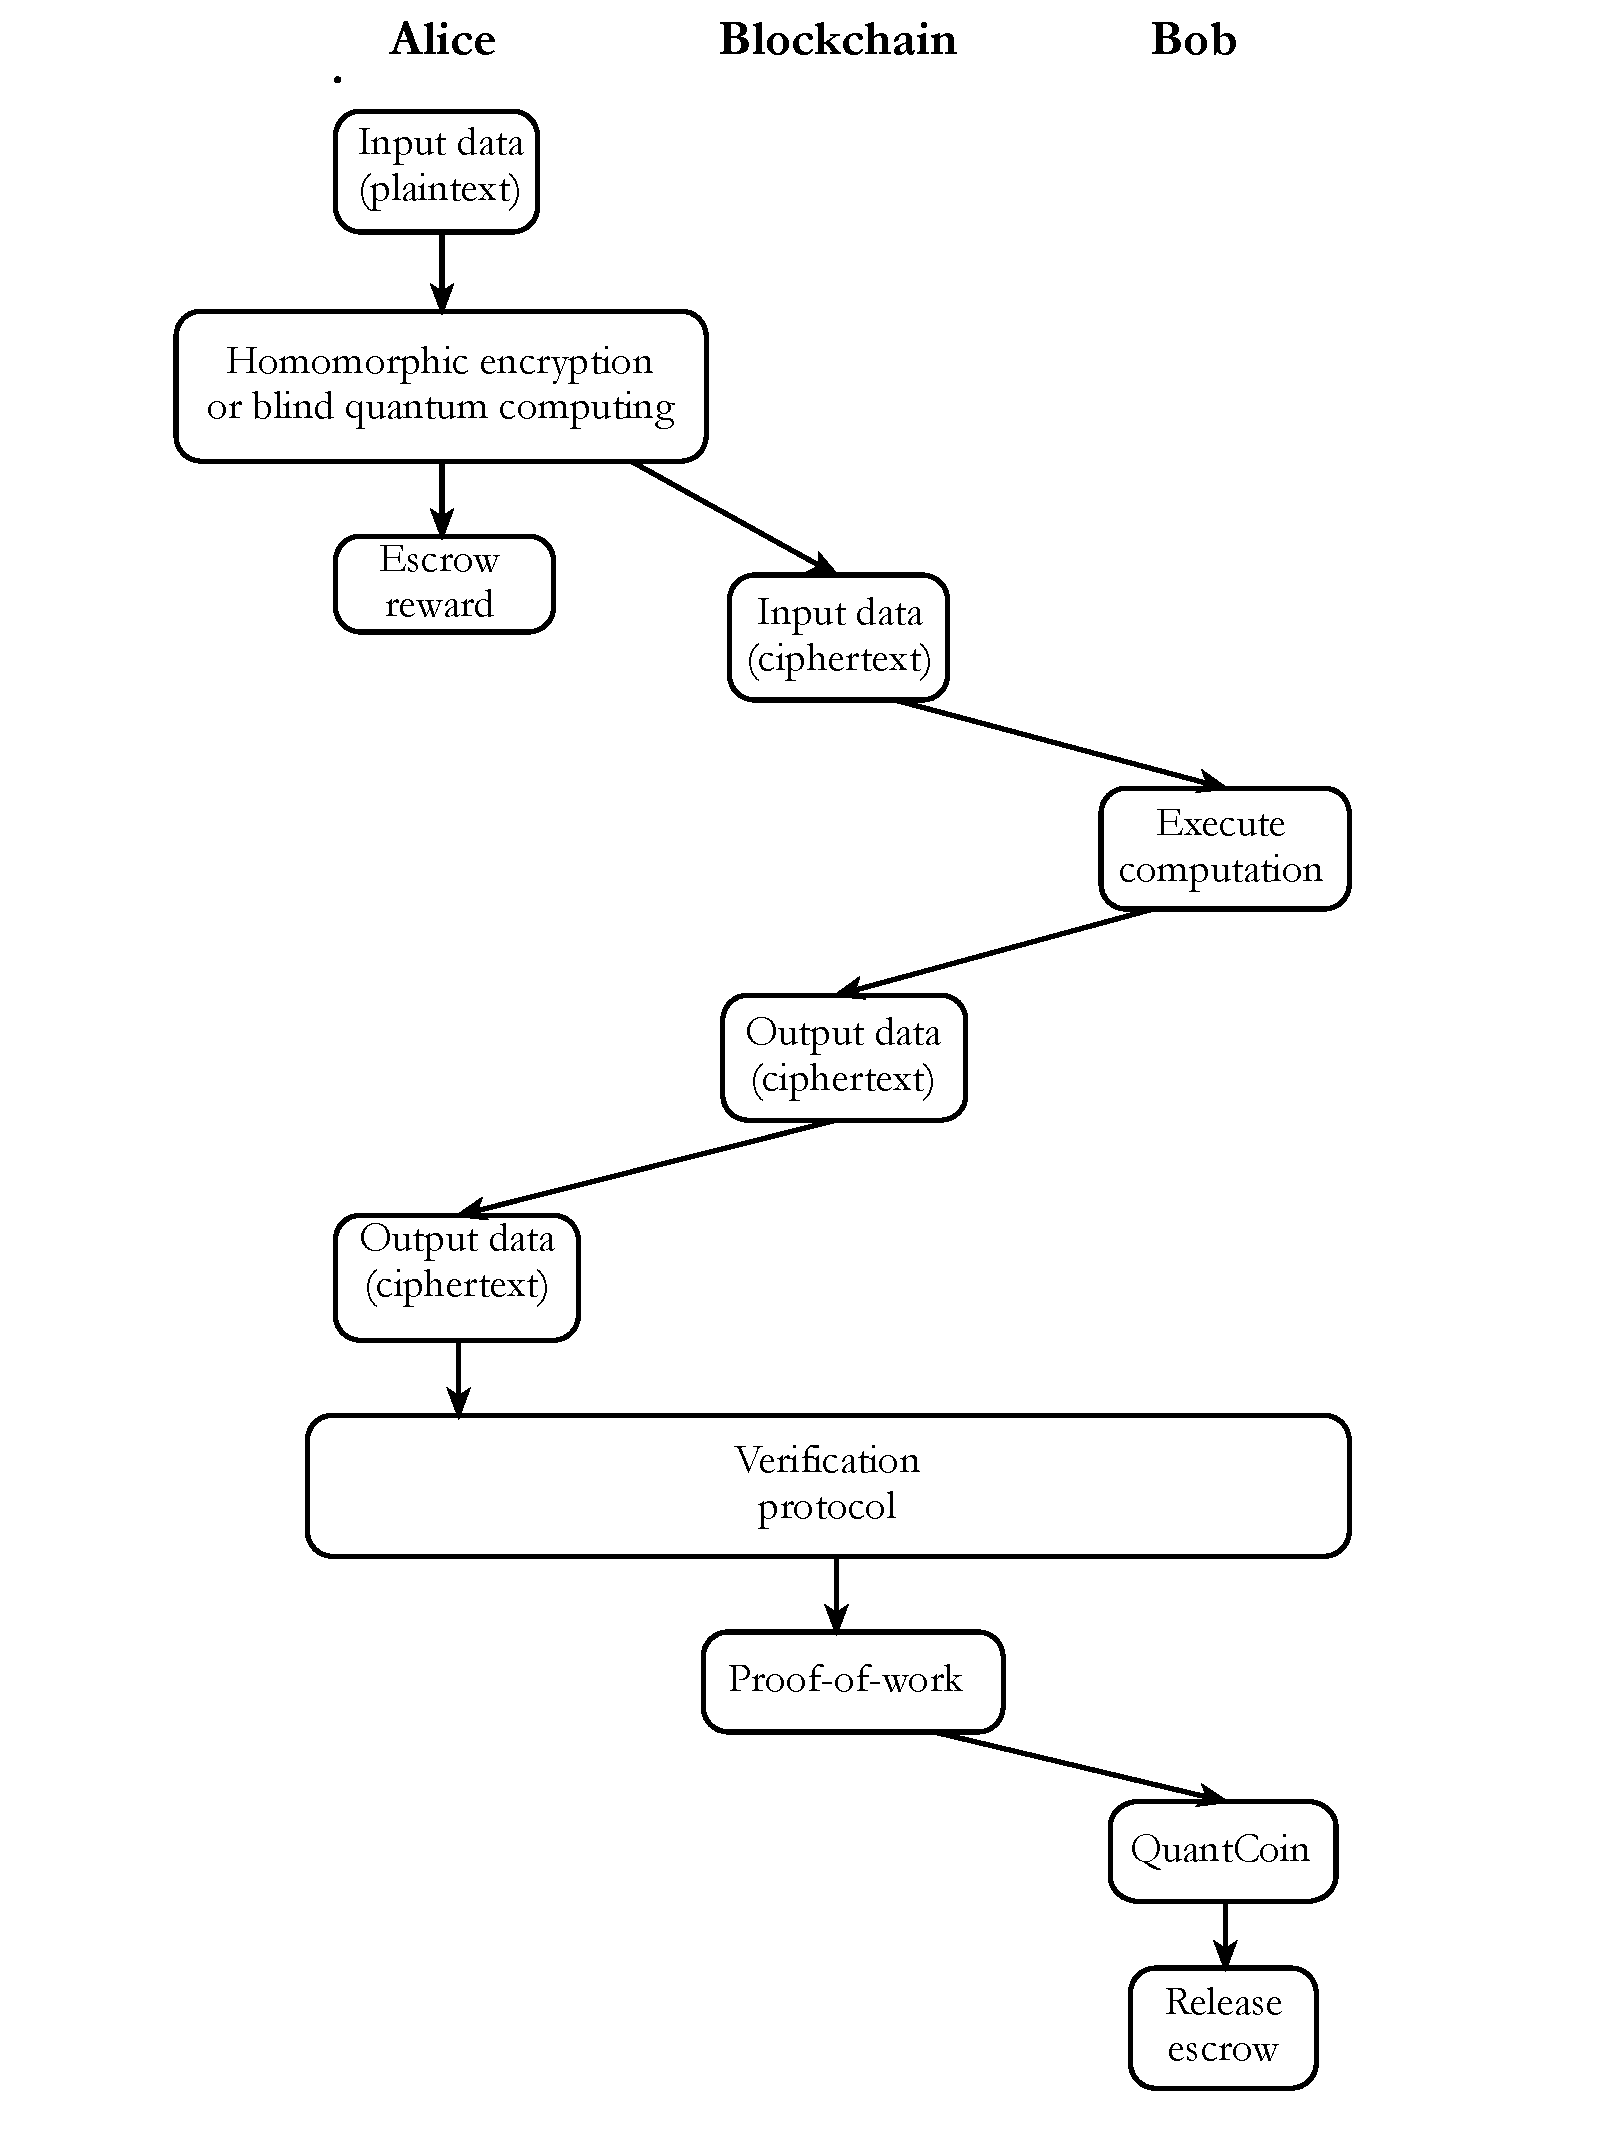
\includegraphics[clip=true, width=0.475\textwidth]{quantcoin_protocol}
\captionspacefig \caption{Flowchart for the QuantCoin\texttrademark\, protocol, introduced in Alg.~\ref{alg:quant_coin}.}\label{fig:quantcoin_protocol}	
\end{figure}

It is evident from the flow of Alg.~\ref{alg:quant_coin} that the mining process now comprises solving an actual quantum computation of intrinsic value to Alice, since she is exchanging assets (e.g dollars or already-existing QuantCoins\texttrademark) in exchange for the computation. Completion of the computation followed by successful verification then further rewards Bob with a fresh QuantCoin\texttrademark\, courtesy of the distributed Blockchain algorithm.

The described protocol, in addition to mining a new coin, associated with the execution of a computation, acts as a currency converter for converting traditional assets (e.g dollars) into QuantCoins\texttrademark. This ability to currency convert is necessary, and completely differs from the original Bitcoin mining process, where coins are fabricated out of thin air by anyone and everyone, independent of their pre-existing monetary wealth -- Bitcoins are not created via conversion from any existing asset, they are an entirely new asset class of their own. The fact that the computation associated with each QuantCoin\texttrademark\, is of intrinsic value on the other hand, implies that Alice ought to be paying something for the service.

Note that we observe an expansion in the money supply with each successfully executed and verified computation -- one additional unit of QuantCoins\texttrademark\, is mined for every unit of computation implemented\footnote{To provide an analogy with the gold standard\index{Gold standard}, think of the physical quantum computer as the goldmine, and each unit of gold it produces as being a QuantCoin\texttrademark. The production of each unit of gold is associated with the utilisation of the mine for a particular amount of time, but the mine can in principle operate indefinitely, with no hard upper-bound on its total future gold yield.}. Unlike Bitcoin, there is no inherent theoretical upper limit on the number of coins that can exist. However the QuantCoin\texttrademark\, money supply\index{Money supply} will be limited for the practical reason that mining each one is associated with a monetary transaction between Alice and Bob, and Alice will eventually run out of assets to exchange for computations.

What relationships characterise the value of QuantCoins\texttrademark? First, in a perfectly efficient market (Sec.~\ref{sec:eff_markets}) we have,
\begin{align}\label{eq:value_quantcoins}
	P_\mathrm{coin} + P_\mathrm{reward} = P_\mathrm{exec},
\end{align}
where, 
$P_\mathrm{coin}$ is the dollar value of a QuantCoin\texttrademark\,, $P_\mathrm{reward}$ is the dollar value of the reward paid by Alice for execution, and $P_\mathrm{exec}$ is the dollar value of cost of execution for Bob.
 
Alternately, rather than Alice paying Bob's reward in dollars, she might pay for them in already-existing QuantCoins\texttrademark. Suppose Alice pays $\lambda$ QuantCoins\texttrademark\, as Bob's reward. Then Eq.~(\ref{eq:value_quantcoins}) reduces to,
\begin{align}
P_\mathrm{coin} =\frac{1}{\lambda+1}P_\mathrm{exec},
\end{align}
providing us with a simple financial model relating the market price of QuantCoins\texttrademark\, and the monetary cost of execution of computations.

Note that with exception to the scenario where Alice buys into QuantCoins\texttrademark\, using dollar currency (or any non-electronic asset that cannot be committed to the Blockchain), the entire protocol is self-enforcing via programmed Blockchain transactions. Bob doesn't get paid his newly earned and freshly printed QuantCoin\texttrademark\, until the verification of the computation has completed and the proof committed to the Blockchain. He therefore cannot get paid until he has executed the computation he promised to, and proven to the network that he actually did.

The main security risk is that of Bob taking Alice's dollars and running, upon receiving the upfront reward in dollars, which necessarily don't reside on the Blockchain since they are not crypto-assets. This could be addressed by introducing trusted third-party escrow agents into the protocol, as method currently used in some online dark markets\index{Dark markets}. 

However, if the upfront payment were being made in pre-existing QuantCoins\texttrademark\,, the Blockchain might be programmed to not release the reward until completion of the final verification stage of the protocol -- effectively an escrow programmed directly into the Blockchain for self-execution. Such self-executing smart-contracts are already a feature in some cryptocurrencies such as Ethereum\index{Ethereum}.

%
% Futures Market Model
%

\subsection{Futures market model}

As described above, the cryptocurrency is effectively backed by the spot market in computation -- we exchange currency for the execution of computations \textit{immediately}. However, one might also envisage more complex cryptocurrencies being backed by the futures market in the licensing of quantum compute-time.

Intuitively, one would expect such a form of cryptocurrency to be sounder than the one backed by the spot market. This is because our spot market-derived coins, once mined are not guaranteed to be convertible to anything of value, including computations. Recall that the execution of the computation takes place immediately when the coin is created.

On the other hand, a QuantCoin\texttrademark\, backed by a guarantee to access quantum compute-time at a designated point in the future necessarily has value, so long as the demand for compute-time does, and maintains value until the contract matures and converts into compute-time at which point it becomes worthless.

We leave explicit construction of a futures-based QuantCoin\texttrademark\, model as an exercise for the interested reader, primarily because we haven't thought it through properly\index{Laziness}.

%
% Economic properties of the qubit marketplace
%

\section{Economic properties of the qubit marketplace}\index{Economic properties}\label{sec:econ_prop}

\dropcap{T}{he} development and implementation of the quantum internet will give rise to a new tradable commodity -- the qubit. The pricing mechanisms associated with a qubit market were explained earlier in this part. Here we provide a broader discussion on the economic properties of such a marketplace. The are two areas of particular interest we will focus on:
\begin{enumerate}
	\item The responsiveness of the qubit market to price fluctuations, measured by elasticity.\index{Elasticity}
	\item The implications of qubit market properties for broader society in terms of pricing and taxation.\index{Taxation}
\end{enumerate}

\subsection{The concept of elasticity}\index{Elasticity}

Elasticity as a concept is measured through percentage changes. Starting with the demand for qubits as an example, the \textit{elasticity of demand}\index{Elasticity}, $E_d$, is the percentage change in the quantity demanded of a good, divided by the percentage change in the price of a good. Mathematically, the elasticity of demand is represented as,
\begin{align}\index{Elasticity!Formula}
E_d = \frac{\% \Delta Q_d}{\% \Delta P}.	
\end{align}

From this relationship, inferences about the underlying commodity can be made, summarised as follows:
\begin{itemize}
	\item \mbox{$|E_d|>1$}: the percentage change in quantity is greater than the percentage change in price, and is therefore \textit{elastic}. This indicates that demand for the asset in the market is responsive to small price changes.
	\item \mbox{$|E_d|<1$}: there is a proportionally larger change in price, for a smaller shift in demand. This indicates that demand is less responsive to price changes, and considered \textit{inelastic}.
	\item \mbox{$|E_d|=1$}: we have \textit{unit elasticity}, where the percentage change in quantity demanded is equal to the percentage change in market price.
\end{itemize}

Elasticity of demand is just one context where the concept of elasticity can be applied. Other contexts include: the elasticity of supply, measuring the supply side responsiveness to changes in price; income elasticity, which captures how the quantity of goods in the market change relative to changes in the income of consumers; and cross-price elasticity, which compares the percentage change in quantity of one good, relative to the percentage change in price of another good. An example that we will come back to is how changes in the price of quantum computing may have an effect on the quantity demanded of high-performance classical computing (i.e conventional supercomputing).

\subsection{Elasticity of the qubit market}\index{Elasticity!Qubits}

A number of factors will affect the elasticity of demand and supply in the qubit market. The most significant factor affecting the demand for qubits is the availability of substitutes\index{Substitution}. Given that quantum processing can efficiently solve unique problems that classical computing cannot, there are no close substitutes for qubits -- a transistor is no substitute for a qubit! Consequently, elasticity of demand will be relatively inelastic: the quantity of qubits demanded will be relatively unresponsive to price fluctuations and changes, since there are no viable alternatives to substitute with. 

The supply side of the equation is also initially going to be highly inelastic. However, as time progresses and technological advancements and enhancements increase the computational power of the quantum internet, the supply of qubits will become increasingly responsive to price fluctuations \comment{Why?}. However, the extent to how elastic the supply becomes over time is also going to be affected by potential for excess capacity given the exponential trajectory of the manufacture of qubits as new and improved fabrication technologies emerge -- the quantum Moore's Law\index{Quantum Moore's Law}.

%
% Economic Implications
%

\section{Economic implications}

\dropcap{O}{ur} analysis thus far has been very theoretical. But our observations have very tangible implications in the real world. This has implications for governments, regulatory authorities, fiscal and technology policy, national security, and any end users of the quantum cloud.

%
% The Price To Pay For Isolationism
%

\subsection{The price to pay for isolationism}\index{Isolationism}

In many traditional sectors of the economy there is an economic incentive to directly compete against other market participants. However in the quantum era the incentive is for owners of quantum computing hardware to cooperate and contribute their resources to the quantum internet rather than go it alone, as a direct consequence of super-linear leverage.

Only those hardware owners who unite with the global network will benefit from its leverage and remain competitive. Those who choose not to participate in the global network will be priced out of the market via exponentially higher cost per FLOP (assuming all other costs are equal).

This effectively taxes the cost of computation for those who fail to unify their assets with the network. And it is in the direct economic self-interest of all market participants to contribute their resources to the time-shared quantum cloud.

%
% Taxation
%

\subsection{Taxation}\label{sec:taxation}\index{Taxation}

Any asset, dividend, derivative or other financial instrument will inevitably be subject to taxation. Any form of taxation has multiplier effects as the cost markup is repeatedly handed from one market participant to the next, influencing the chain of supply and demand along the way. However, this multiplier and other economic consequences are highly dependent on the asset undergoing transaction -- the economic implications of personal income tax are quite different to those of capital gains tax!

\subsubsection{Computational perspective}

We now consider the effect of taxation on quantum resources, specifically in the form of a \textit{qubit tax}\index{Taxation} -- a sales tax on the purchase of physical qubits. Although this model of taxation is unlikely to be implemented as we describe, it serves as an insightful test-bed for thought experiments into the qualitative implications of taxing quantum assets.

Imagine that consumers have an amount of capital available for the purchase of qubits. Let $\gamma_T$ be the rate of taxation (\mbox{$\gamma_T=1$} represents no taxation, \mbox{$\gamma_T>1$} represents positive taxation, and \mbox{$\gamma_T<1$} represents subsidisation). Then the cost of physical qubits is marked up by $\gamma_T$, reducing the number of qubits that can be afforded by the consumers to (assuming fixed capital available for purchasing),
\begin{align}
	N_\mathrm{tax} = \frac{N_\mathrm{no\,tax}}{\gamma_T}.
\end{align}

We now wish to understand how this taxation influences the computational power of the network. We define the \textit{tax performance multiplier}\index{Tax performance multiplier},
\begin{definition}[Tax performance multiplier]
The \textit{tax performance multiplier}\index{Tax performance multiplier}, is the ratio between computational scaling functions with and without qubit taxation,
\begin{align}
M(N_\mathrm{tax}) &= \frac{f_\mathrm{sc}(N_\mathrm{tax})}{f_\mathrm{sc}(N_\mathrm{no\,tax})} \nonumber \\
&= \frac{f_\mathrm{sc}(N_\mathrm{tax})}{f_\mathrm{sc}(N_\mathrm{tax} \gamma_T)},\nonumber\\
M^\mathrm{dB}(N_\mathrm{tax}) &= 10\log_{10}(M(N_\mathrm{tax})),
\end{align}
where the consumers have purchased $N_\mathrm{tax}$ qubits, after taxation, at a markup rate of $\gamma_T$.
\end{definition}
The tax performance multiplier effectively gives us a factor by which computational power is depreciated under taxation. We can accomodate for other models of taxation and regulation by choosing an appropriate relationship between $N_\mathrm{tax}$, $N_\mathrm{no\,tax}$, and the taxation and regulatory framework.

Using our illustrative examples of computational scaling functions (linear, polynomial and exponential), the respective tax performance multipliers are given by,
\begin{align}
M_\mathrm{linear}(N_\mathrm{tax}) &= \frac{1}{\gamma_T}, \nonumber \\
M_\mathrm{poly}(N_\mathrm{tax}) &= \frac{1}{{\gamma_T}^p}, \nonumber \\
M_\mathrm{exp} (N_\mathrm{tax}) &= e^{N_\mathrm{tax}(1-\gamma_T)}.
\end{align}

This demonstrates that the computational power of classical networks is simply inversely proportional to the rate of taxation, i.e a linear tax performance multiplier, as we intuitively expect. And for quadratic scaling functions the dependence is inverse quadratic in the taxation rate. In both cases the multiplier is a constant factor, independent of the network size. However, for exponential scaling functions we observe an exponential dependence on both the rate of taxation and the size of the network, shown in Fig.~\ref{fig:tax_exp}. Note that for large networks, executing computations with exponential scaling functions, there is enormous sensitivity to variations in tax rates, yielding very high leverage in computational return by tax rates.

This implies that as the quantum network expands over time, its joint processing power decreases exponentially with the rate of taxation, yielding an ever-decreasing performance multiplier. In Sec.~\ref{sec:economics} we discuss some of the implications of this uniquely quantum phenomena.

However, taxation could also be negative, in the form of subsidisation. In Fig.~\ref{fig:tax_exp} we focus on the region surrounding neutral taxation, showing small degrees of taxation and subsidisation on either side. Evidently, even small degrees of subsidisation have a very strong impact on the performance multiplier (more pronounced than the same rate of positive taxation!). This makes subsidisation of qubit expansion highly tempting.

\if 2\pubmode
\begin{figure}[!htbp]
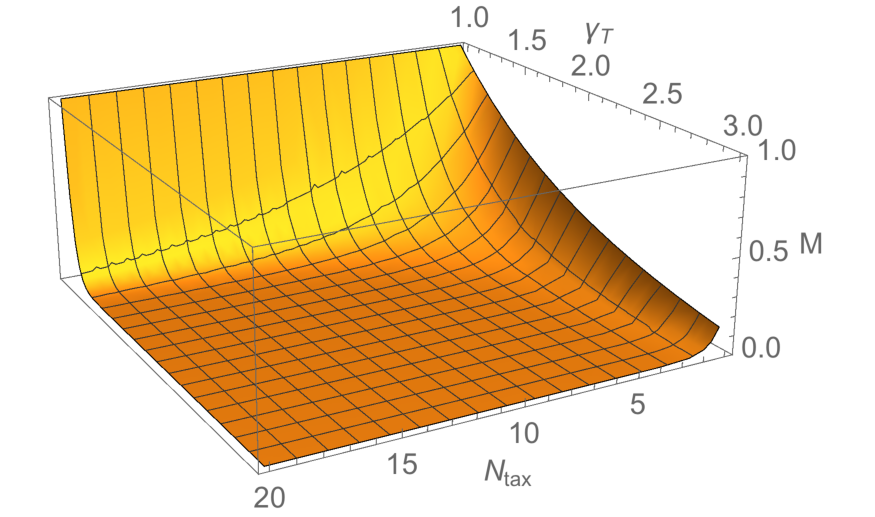
\includegraphics[clip=true, width=0.475\textwidth]{tax_exp}\\
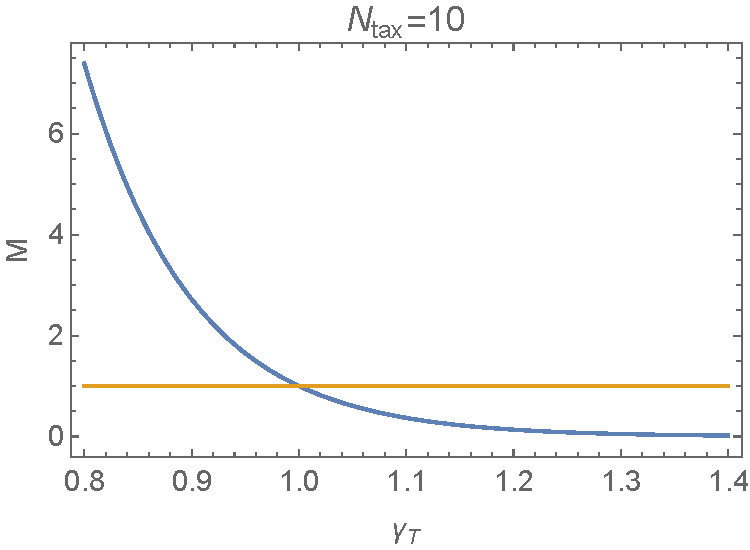
\includegraphics[clip=true, width=0.475\textwidth]{tax_subsidy}
\captionspacefig \caption{(top) Relationship between the tax performance multiplier, (positive) tax rate, and network size, assuming an exponential computational scaling function, in the regime of positive taxation, \mbox{$\gamma_T>1$}. (bottom) For \mbox{$N_\mathrm{tax}=10$}, a zoom into the region around neutral taxation, where \mbox{$\gamma_T\approx 1$}, showing slight degrees of both taxation (\mbox{$\gamma_T>1$}) and subsidisation (\mbox{$\gamma_T<1$}). Neutral taxation, \mbox{$\gamma_T=1$}, is shown in orange.}\label{fig:tax_exp}\index{Tea party}\index{Don't tread on me}
\end{figure}
\else
\begin{figure*}[!htbp]
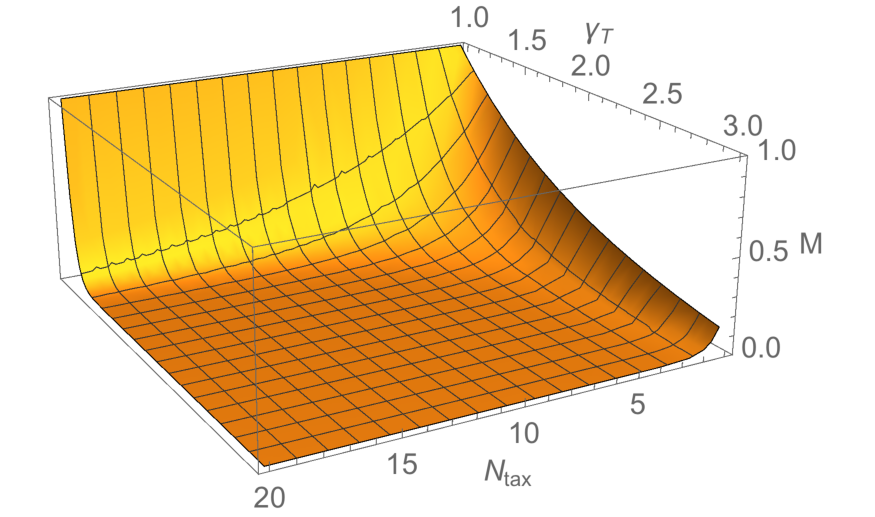
\includegraphics[clip=true, width=0.475\textwidth]{tax_exp}
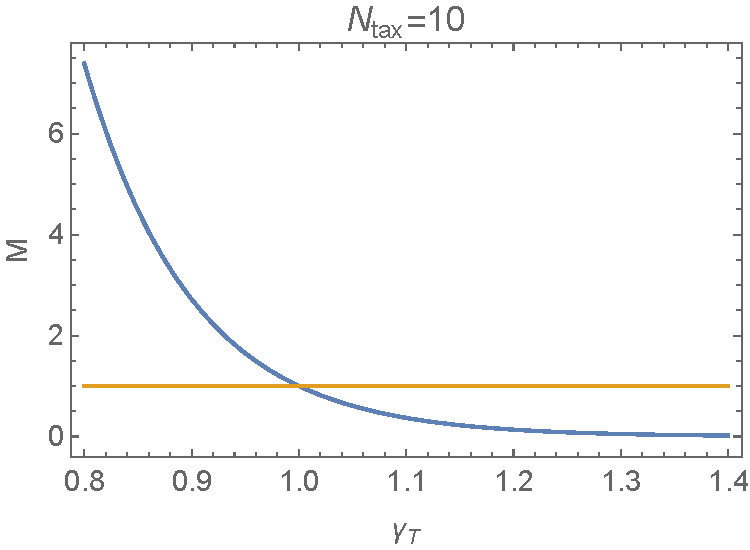
\includegraphics[clip=true, width=0.475\textwidth]{tax_subsidy}
\captionspacefig \caption{(left) Relationship between the tax performance multiplier, (positive) tax rate, and network size, assuming an exponential computational scaling function, in the regime of positive taxation, \mbox{$\gamma_T>1$}. (right) For \mbox{$N_\mathrm{tax}=10$}, a zoom into the region around neutral taxation, where \mbox{$\gamma_T\approx 1$}, showing slight degrees of both taxation (\mbox{$\gamma_T>1$}) and subsidisation (\mbox{$\gamma_T<1$}). Neutral taxation, \mbox{$\gamma_T=1$}, is shown in orange.}\label{fig:tax_exp}\index{Tea party}\index{Don't tread on me}
\end{figure*}
\fi

\subsubsection{Policy perspective}\index{Policy}\label{sec:policy}

Irrespective of the magnitude of change, the elasticities, especially on the demand side, indicate that the qubit would be ripe for the application of a consumer-driven tax. Graphically the imposition of a tax within a perfectly competitive market would take on the form of Fig.~\ref{fig:supply_demand}(a)\index{Supply \& demand curve}.

\if 2\pubmode
\begin{figure}[!htbp]
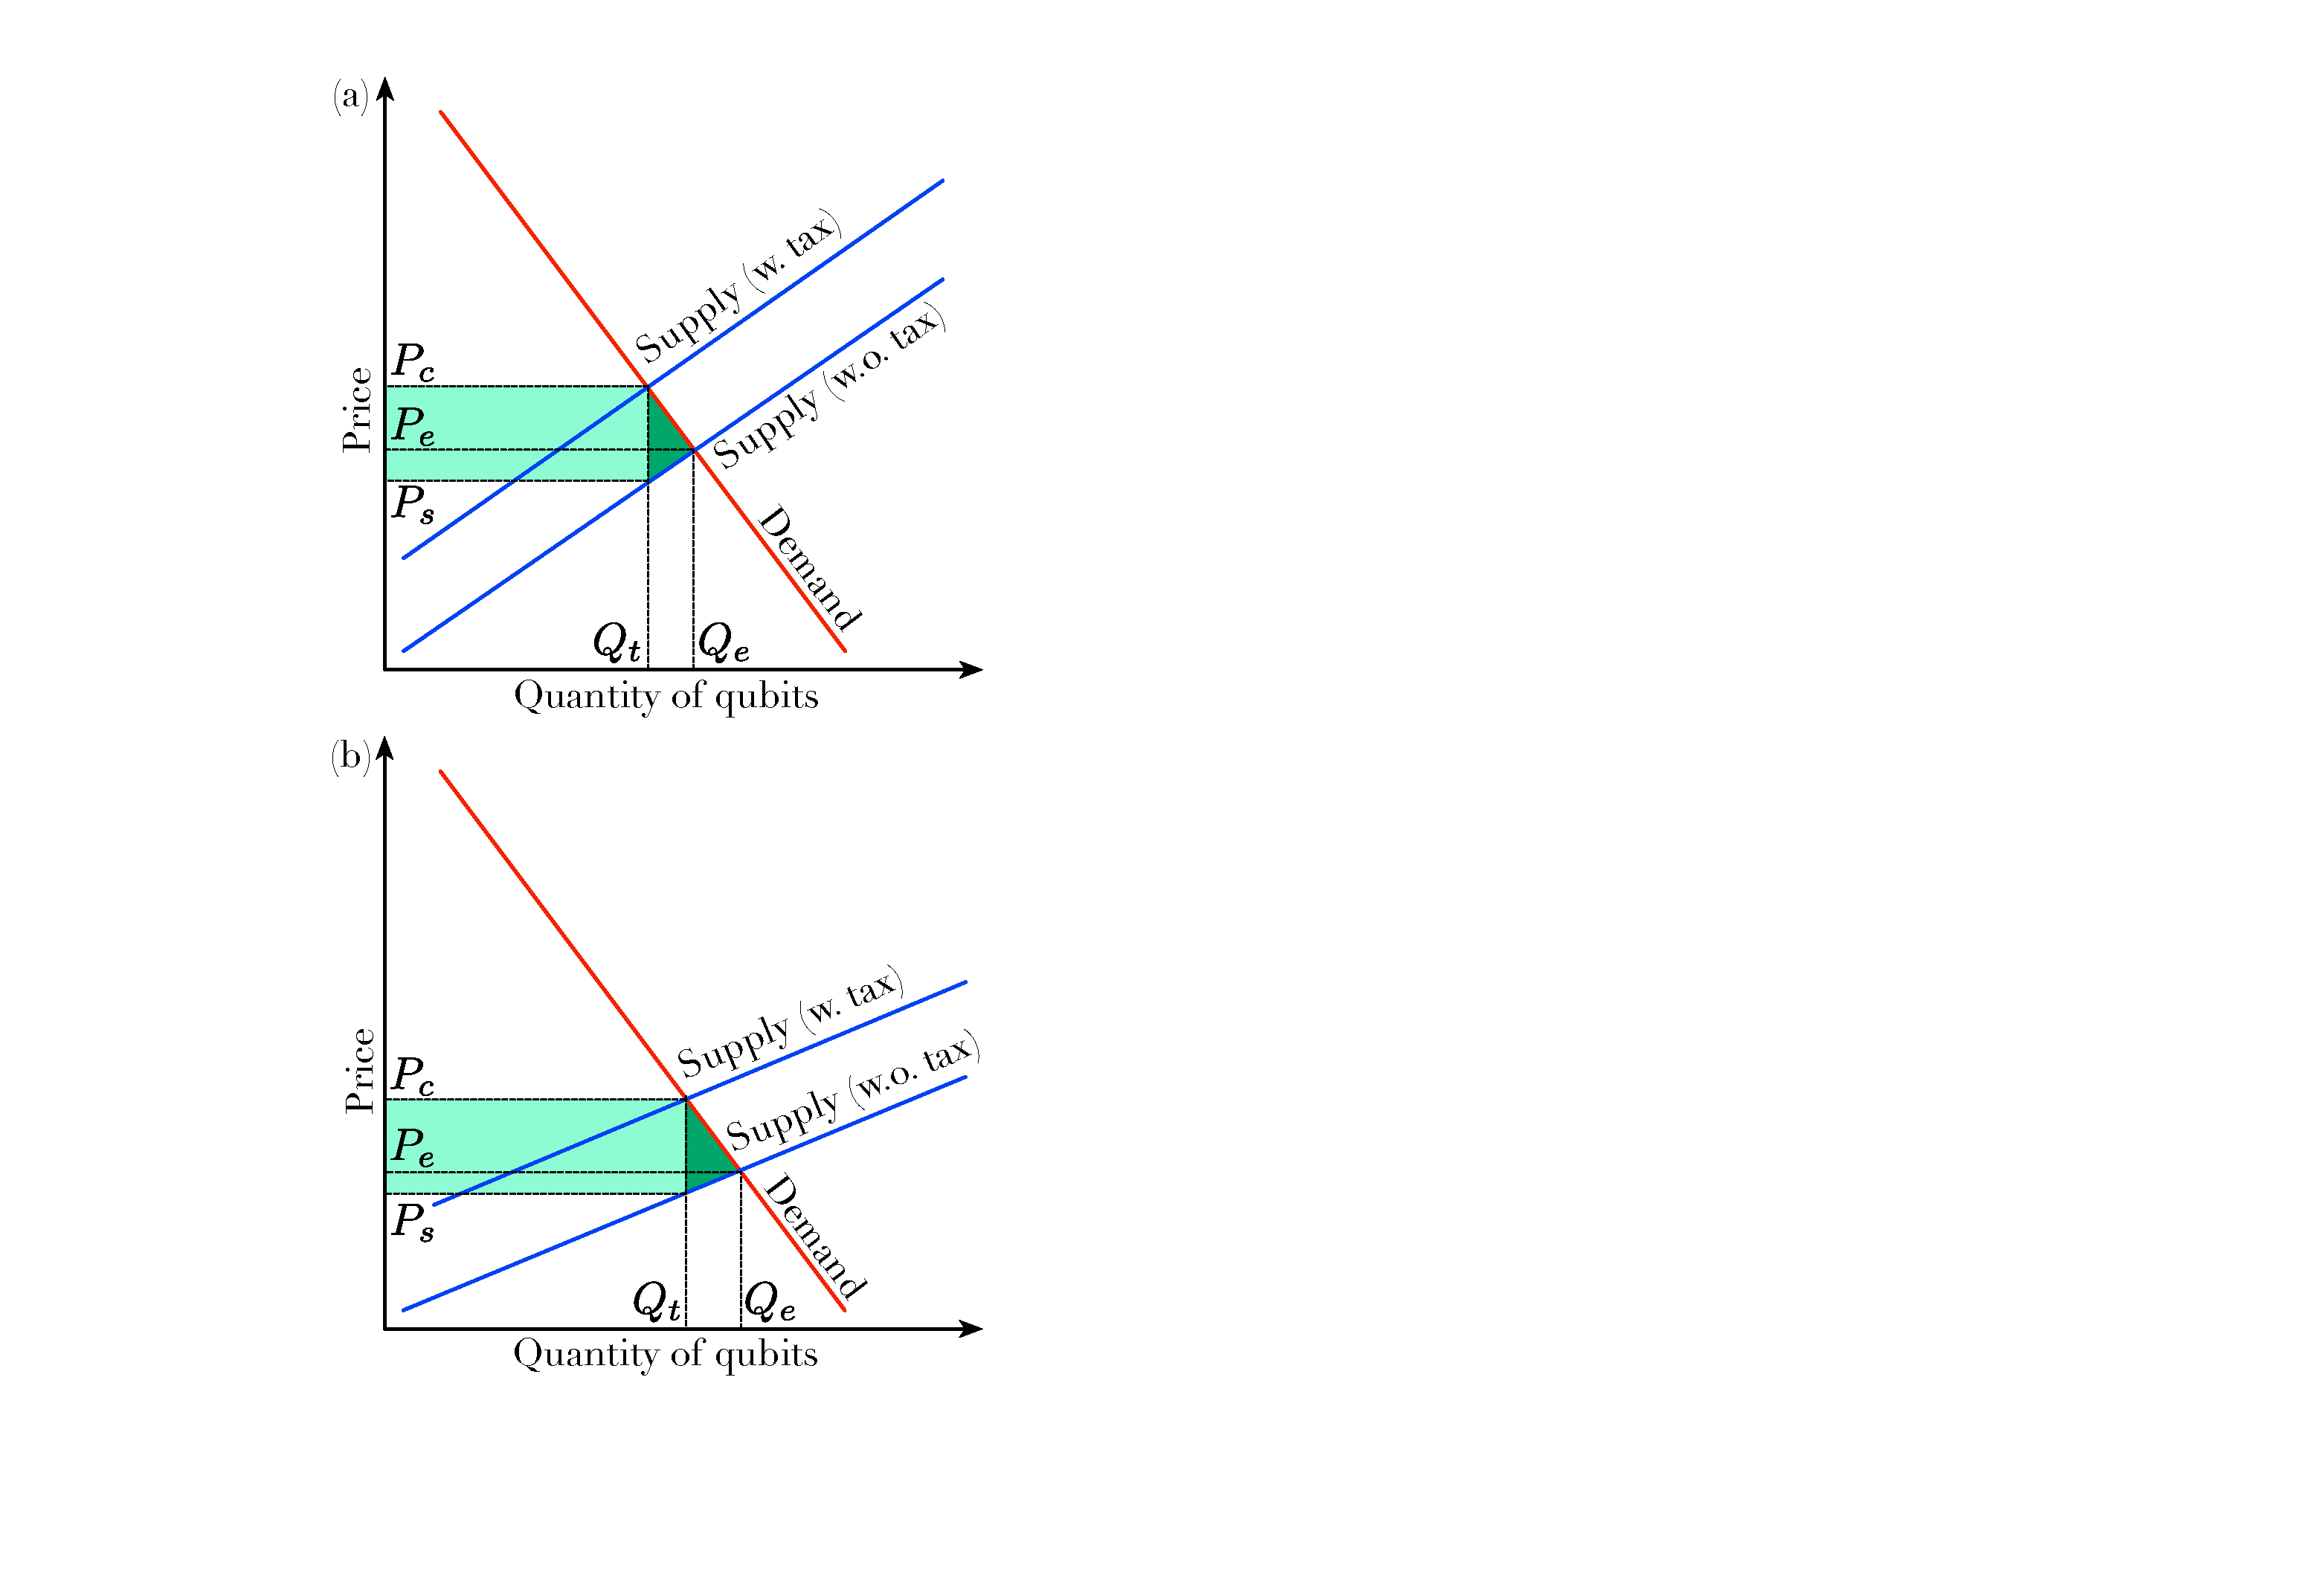
\includegraphics[clip=true, width=0.45\textwidth]{supply_demand_long}
\captionspacefig \caption{Hypothetical supply/demand curves, showing the impact of taxation on price and supply, for both inelastic (a) and elastic (b) market dynamics. $Q_e$ and $P_e$ are the efficient market quantity and price of the asset respectively. $P_s$ is the price faced by suppliers, while $P_c$ is the consumer price under taxation. $Q_t$ is the quantity in a taxed environment. The net tax revenue collected is shaded in light teal, and the loss of market efficiency through the imposition of taxation is shaded in dark teal.}\index{Supply \& demand curve}\label{fig:supply_demand}	
\end{figure}
\else
\begin{figure*}[!htbp]
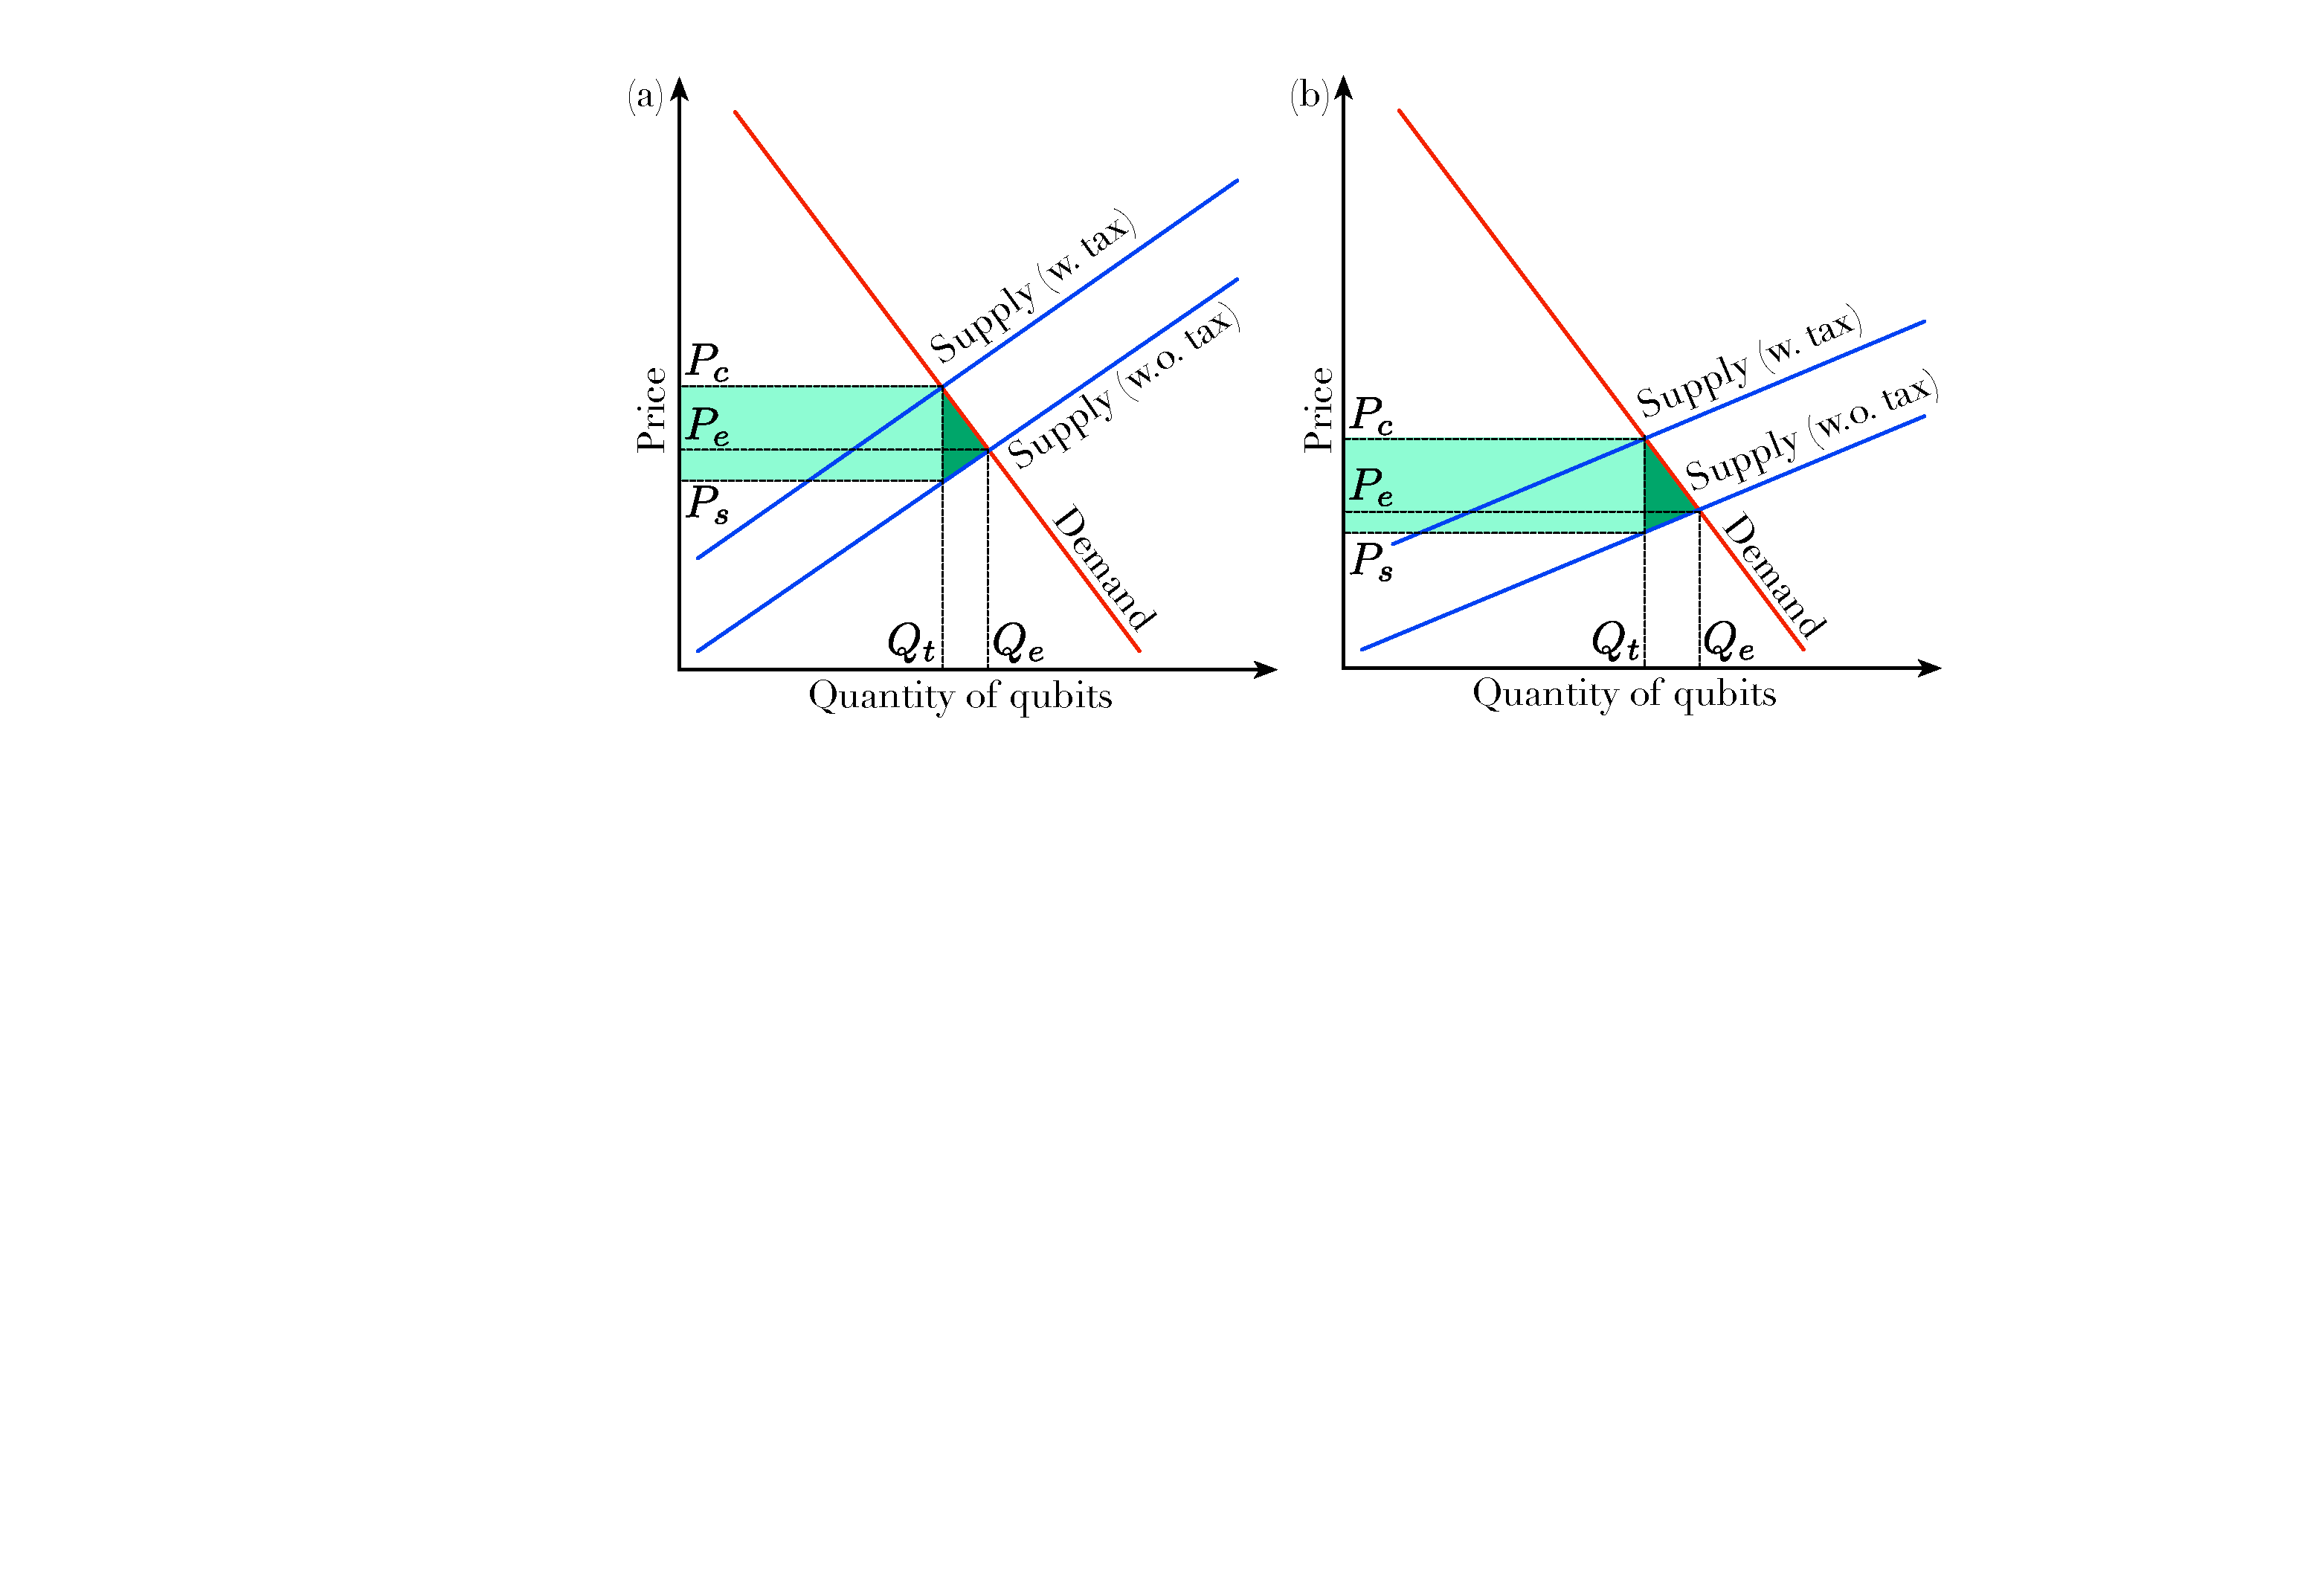
\includegraphics[clip=true, width=0.8\textwidth]{supply_demand}
\captionspacefig \caption{Hypothetical supply/demand curves, showing the impact of taxation on price and supply, for both inelastic (a) and elastic (b) market dynamics. $Q_e$ and $P_e$ are the efficient market quantity and price of the asset respectively. $P_s$ is the price faced by suppliers, while $P_c$ is the consumer price under taxation. $Q_t$ is the quantity in a taxed environment. The net tax revenue collected is shaded in light teal, and the loss of market efficiency through the imposition of taxation is shaded in dark teal.}\index{Supply \& demand curve}\label{fig:supply_demand}	
\end{figure*}
\fi

The graph indicates a downward sloping demand line, indicating that the lower the price, the higher the demand. The upward sloping supply curve reflects financial incentive, the higher the price, the greater the incentive there is for firms to increase the quantity of qubits available to the market. Correlating this to elasticities, a steeper demand or supply curve indicates a higher degree of inelasticity. As such, in Fig.~\ref{fig:supply_demand}(a)\index{Supply \& demand curve}, the slope of both the demand and supply curves are relatively inelastic (compared to a $45^\circ$ reference line). From this, the imposition of a consumer-based tax can be shown through the vertical shift of the supply curve, with the magnitude of the shift, \mbox{$P_c - P_s$}, indicating the per-qubit value of the tax. Other important observations from the graph are the tax revenue\index{Tax revenue} collected (shaded in light teal), the loss of market efficiency\index{Market efficiency} through the imposition of a tax (shaded in dark teal), and a relatively small reduction in the quantity of qubits offered on the market from the efficient quantity, $Q_e$, to the quantity with the consumer tax, $Q_t$\index{Taxation}. 

An important implication of the imposition of the tax is the share of the taxation burden\index{Taxation}. The change in price from the efficient price, $P_e$, to the new market price faced by consumers, $P_c$, is somewhat equivalent to the shift from $P_e$ to the price point that the suppliers of qubits will receive, $P_s$. This means that the tax burden is likely to be equally shared between producers and consumers, which in the long term could act as a disincentive for increased production.

Fig.~\ref{fig:supply_demand}(b), however, shows a longer-term view of the qubit market, where the supply of qubits has become more elastic in nature. That is, the quantity supplied to the market becomes more sensitive to price fluctuations. This change in elasticity results in a shift in the tax burden, with a greater proportion of the tax now being paid by consumers, with only a small shift from the efficient price, $P_e$, to the price suppliers will face, $P_s$. 

From a policy implications perspective, this means that governments wanting to cash in on the new technology need to be cautious with the imposition of taxes relative to market maturity. Imposing a significant tax early on may only act as a disincentive to the development of the industry. However, once the market matures further, the imposition of a qubit tax would make strong economic sense, as there will be minimal loss of market efficiency. Importantly, such a tax on computational power alone could serve to be a relatively stable revenue generation tool for governments. 

%
% Game theory of the qubit
%

\subsection{Game theory of the qubit}\index{Game theory}\label{sec:game_theory}

Previously we discussed the implications of the imposition of taxation on the qubit market, assuming it operates in a relatively competitive environment. However, given the massive technological and financial investment made to realise just a single quantum computing system, let alone an entire network, the likely resulting market structure will not be a perfectly competitive one. Rather, just a few significant firms will likely dominate the space, creating a global oligopoly where profit extraction in the face of various taxation frameworks is to be the more likely scenario. 

This then leads to game theory, which can make a significant contribution to our understanding of how a potential qubit market is not only likely to operate, but more importantly, that the suppliers of qubits will be engaging in a cooperative game with each other to maximise their utility (profits), while governments will be engaging in a competitive game with other governments with a clear objective: maximise taxation revenue, while not ceding ground to competing countries in hosting qubits. The following sections will discuss these games and provide an indication of how various strategies perform in terms of cooperation and competition.

\subsubsection{The Nash equilibrium \& VNM solution for maximal utility}\index{Nash equilibrium}

\comment{To do}

%
% Regulatory Frameworks
%

\subsection{Regulatory frameworks} \index{Regulatory frameworks}

\comment{To do. How will leverage asymmetry affect regulatory frameworks, defence export laws etc.}

%
% Subjective vs Objective Value of Computation
%

\subsection{Subjective vs. objective value of computation}\index{Subjective value of computation}\index{Objective value of computation}\label{sec:sub_vs_obj}

As discussed in relation to combined computational scaling functions (Sec.~\ref{sec:comb_comp_sc_func})\index{Combined computational scaling functions}, different market participants will be executing different software applications on their share of the quantum computing resources, with differing QCLs\index{Quantum computational leverage}. Because the applications differ between users, as do their QCLs, so too does the monetary value of the computations they are performing. This yields the distinction between \textit{subjective}\index{Subjective value of computation} and \textit{objective}\index{Objective value of computation} value of computation:

\begin{itemize}
\item Subjective value of computation: the value to an end-user of a computation, measured in terms of their associated monetary profit from utilising its output, which is highly application-specific.
\item Objective value of computation: the cost of the physical hardware and infrastructure, which is not application-specific, but rather stipulated by technological and manufacturing progress.
\end{itemize}

This effectively implies that some users pay more for computation (in terms of return on investment\index{Return on investment (RoI)}) than others. While the objective cost of computation is conceptually simple to model (as performed in a rudimentary fashion in Sec.~\ref{sec:cost_of_comp}), the subjective cost is a highly non-trivial one. It will depend heavily on the scaling function of the algorithm run by a user, and of course the economic objectives of their computation -- a quantum simulation algorithm executed by an R\&D lab\index{R\&D} is likely to be of greater monetary value than and undergrad using his university's resources to execute the same task for completing an assignment!

%
% The Quantum Stockmarket
%

\subsection{The quantum stock market}\index{Quantum stock market}

In light of the distinction between subjective and objective value of computation, the question  is how to reconcile this distinction in value, given the diversity of applications in the quantum marketplace. This will supersede the na\"ive models for cost of computation presented earlier, which were based entirely on objective value. Of course, subjective value is what people are actually willing to pay for in the real-world!

This will give rise to a marketplace for tradable units of quantum computation, where the underlying asset is time-shares in the global network. We refer to this as the \textit{quantum stock market} -- a marketplace subject to ordinary supply and demand, economic, and of course psychological pressures. In a scenario where a large number of users are executing computations with high return (think the R\&D lab), asset values will be traded up. Contrarily, in a scenario of low-return computations (think our poor undergrad), they will be traded down. These market forces will be highly time-dependent, varying against many other factors in the economy, such as the emergence of new applications for quantum computation -- the discovery of an important new algorithm could spontaneously distort the market leading to major corrections.

The relative market value of computation will subsequently drive the direction of investment into quantum hardware, with carry-over effects on future market prices. If investment stagnates, so too will growth in computational dividends, driving up market rates by limiting supply (assuming positive growth in demand). This will, after market adjustment, drive investment back into the system to satisfy increasing demand. Thus, despite the present uncertainty into the future dynamics of the quantum stock market, we expect this positive feedback loop to ensure consistent, ongoing investment into the quantum network, and at least some marginal degree of price stability.

What is likely to arise is that most owners of quantum hardware will not be consumers, but rather investors, potentially highly speculative ones, who float their resources on the quantum stock market, betting on changes in demand for computation and their associated subjective cost. This trading could involve transactions in the direct underlying asset, future contracts (Sec.~\ref{sec:for_contr}) for locking in required computational power at future points in time, or more complex derivatives. For example, an investor anticipating a surge in high-value computations is likely to invest more heavily into hardware with the expectation of an uptrend in market rates of their licensing. And their return on investment\index{Return on investment (RoI)} will reflect these market dynamics.

As all markets for tradable assets do, sophisticated derivative markets will inevitably emerge, whereby people can speculate on or hedge against market dynamics, taking long, short, or more complex market positions, potentially in a highly-leveraged manner. As discussed in Sec.~\ref{sec:for_contr}, derivatives such as future contracts can be extremely helpful in enabling consumers to lock in future prices, creating a stable and predictable business climate. Similarly, other derivatives will enable market participants to hedge\index{Hedging} other quantum-related investments. For example, suppose an investor held a stake in an R\&D lab, highly reliant on quantum computing resources. By taking a leveraged long position on the market value for computation, he may limit losses on his R\&D investment associated with the higher price (and hence lower profit) they will be paying for computation. No doubt, market manipulation and all the usual nonsense and shenanigans\index{Shenanigans} will ensue.

%
% Geographic Localisation
%

\subsection{Geographic localisation}\index{Geographic localisation}\label{sec:geo_loc}

Because of the resource overheads associated with performing computations in a distributed manner, e.g via the resource costs associated with long-range repeater networks\index{Quantum repeater networks}, there is an economic imperative to localise quantum infrastructure, so as to mitigate this -- there is a clear economic benefit associated with housing qubits in close geographic proximity such that no long-distance quantum channels are required.

However, it's undesirable to \textit{entirely} centralise infrastructure of \textit{any} type, for two primary reasons:
\begin{itemize}
	\item Geostrategic competition\index{Geostrategic politics}: competing nation states or enterprises may not want essential infrastructure to be located entirely offshore, placing them at the mercy of their strategic competitors.
	\item Geographical redundancy\index{Geographic redundancy}: to eliminate single points of failure\index{Single points of failure} (SPOF), which undermine network robustness, it's desirable for infrastructure to be geographically decentralised. In present-day large-scale distributed classical platforms, geographical redundancy is a key consideration. Even though it would be most efficient if all data were completely centralised, obviating communications overheads, it would be catastrophic if a single earthquake (or war!) could decimate the entire system.
\end{itemize}

Thus, we can reasonably anticipate that the quantum internet will not evolve like the classical `internet of things'\index{Internet of things}, whereby a massive number of ultra-small computational resources are scattered across the globe and networked. Rather, a relatively small number of central `hubs'\index{Hubs} are likely to emerge, which centralise enormous computational power, interconnected via the quantum internet to form the globally unified quantum cloud (Sec.~\ref{sec:glob_unif_quant_cloud}).

Much like the classical internet, it's to be expected the network that will emerge will approximate a scale-free network (Sec.~\ref{sec:scale_free_networks})\index{Scale-free networks}, with a very hierarchical structure, following a Pareto distribution\index{Power law} in hub-size.

%
% Summary of Economic Models
%

\section{Summary of economic models}\index{Summary of economic models}\label{sec:summary_economic_models}

\dropcap{I}{n} Table.~\ref{tab:summary_ec_models} we summarise the economic models and parameters we developed, and applied them to several illustrative scaling functions of particular interest: linear, polynomial, and exponential.

\latinquote{Errare humanum est.}

\startnormtable
\renewcommand{\arraystretch}{0.5}

\begin{table*}[!htbp]
{\footnotesize
\begin{tabular}{|m{0.21\linewidth}|m{0.21\linewidth}|m{0.15\linewidth}|m{0.155\linewidth}|m{0.225\linewidth}|}
	\hline
	\[\mathrm{Model}\] & \[\mathrm{General\, form}\] & \[f_\mathrm{sc}(n)=n\] & \[f_\mathrm{sc}(n)=n^p\] & \[f_\mathrm{sc}(n)=e^n\]\\
	\hline \hline
	\begin{flushleft}Per-qubit computational power (Sec.~\ref{sec:NPSF})\end{flushleft} & \[\chi_\mathrm{sc}(n)=\frac{f_\mathrm{sc}(n)}{n}\] & \[1\] & \[n^{p-1}\] & \[\frac{e^n}{n}\]\\
	\hline
	\begin{flushleft}Network power (Sec.~\ref{sec:network_power})\end{flushleft} & \[P(t)=f_\mathrm{sc}(N_0{\gamma_N}^t)\] & \[N_0{\gamma_N}^t\] & \[\left(N_0{\gamma_N}^t\right)^p\] & \[ e^{N_0{\gamma_N}^t}\] \\
	\hline
	\begin{flushleft}Network value (Sec.~\ref{sec:network_value})\end{flushleft} & \[V(t)=C_0 N_0 \left(\frac{\gamma_N}{\gamma_C}\right)^t\] & \[C_0 N_0 \left(\frac{\gamma_N}{\gamma_C}\right)^t\] & \[C_0 N_0 \left(\frac{\gamma_N}{\gamma_C}\right)^t\] & \[C_0 N_0 \left(\frac{\gamma_N}{\gamma_C}\right)^t\] \\
	\hline
	\begin{flushleft}Spot price of computation (Sec.~\ref{sec:cost_of_comp})\end{flushleft} & \[L(0)=\frac{e^{\gamma_\mathrm{ror}} C_0}{\chi_\mathrm{sc}(N_0)}\] & \[e^{\gamma_\mathrm{ror}} C_0\] &  \[\frac{e^{\gamma_\mathrm{ror}}C_0}{{N_0}^{p-1}}\] & \[\frac{e^{\gamma_\mathrm{ror}}N_0C_0}{e^{N_0}}\] \\
	\hline
	\begin{flushleft}Future cost of computation (Sec.~\ref{sec:cost_of_comp})\end{flushleft} & \[L(t)=\frac{e^{\gamma_\mathrm{ror}} C_0{\gamma_C}^{-t}}{\chi_\mathrm{sc}(N_0 {\gamma_N}^t)}
\] & \[e^{\gamma_\mathrm{ror}} C_0{\gamma_C}^{-t} \] & \[ \frac{e^{\gamma_\mathrm{ror}} C_0{\gamma_C}^{-t}}{(N_0 {\gamma_N}^t)^{p-1}}
\] & \[ \frac{e^{\gamma_\mathrm{ror}} C_0N_0 \left(\frac{\gamma_N}{\gamma_C}\right)^t}{e^{N_0 {\gamma_N}^t}}\] \\
	\hline
	\begin{flushleft}Time-share computational power (Sec.~\ref{sec:arb_free_time_share})\end{flushleft} & \[c_n=n \cdot \chi_\mathrm{sc}(n_\mathrm{global})
\] & \[n\] & \[n\cdot{n_\mathrm{global}}^{p-1}\] & \[\frac{n e^{n_\mathrm{global}}}{n_\mathrm{global}}\]\\
	\hline
	\begin{flushleft}Problem size scaling function (Sec.~\ref{sec:prob_sc_func})\end{flushleft} & \[s = f_\mathrm{size}^{-1}(n\cdot \chi_\mathrm{sc}(n_\mathrm{global}))\] & \[\frac{n}{\alpha_\mathrm{size}}\] & \[(n \cdot {n_\mathrm{global}}^{p_\mathrm{sc}-1})^\frac{1}{p_\mathrm{size}}\] & \[\alpha_\mathrm{sc}n_\mathrm{global} + \log(n)\]\[-\log(\alpha_\mathrm{sc}n_\mathrm{global})\] \\
	\hline
	\begin{flushleft}Quantum computational leverage (Sec.~\ref{sec:quant_ec_lev})\end{flushleft} & \[\lambda_n=\frac{\chi_\mathrm{sc}(n_\mathrm{global})}{\chi_\mathrm{sc}(n)}\] & \[1\] & \[\left(\frac{n_\mathrm{global}}{n}\right)^{p-1}\] & \[\frac{n e^{n_\mathrm{global}}}{n_\mathrm{global}e^n}\]\\
	\hline
	\begin{flushleft}Single-qubit leverage (Sec.~\ref{sec:quant_ec_lev})\end{flushleft} & \[\lambda_\mathrm{qubit}=\frac{\chi_\mathrm{sc}(n_\mathrm{global})}{\chi_\mathrm{sc}(1)}\] & \[1\] & \[{n_\mathrm{global}}^{p-1}\] & \[\frac{e^{n_\mathrm{global}-1}}{n_\mathrm{global}}\]\\
	\hline
	\begin{flushleft}Time-dependent leverage (Sec.~\ref{sec:quant_ec_lev})\end{flushleft} & \[\lambda_n(t)=\frac{\chi_\mathrm{sc}(N_0{\gamma_N}^t)}{\chi_\mathrm{sc}(n)}\] &  \[1\] & \[\left(\frac{N_0{\gamma_N}^t}{n}\right)^{p-1}\] & \[\frac{n e^{N_0{\gamma_N}^t-n}}{N_0{\gamma_N}^t}\]\\
	\hline
	\begin{flushleft}Static computational return (Sec.~\ref{sec:static_comp_ret})\end{flushleft} & \[r_\mathrm{static}(t) = n\cdot\chi_\mathrm{sc}(N_t)\] & \[n\] & \[n{N_t}^{p-1}\] & \[\frac{n e^{N_t}}{N_t}\] \\
	\hline
	\begin{flushleft}Forward contract price (Sec.~\ref{sec:for_contr})\end{flushleft} & \[F(T)=\frac{e^{\gamma_\mathrm{ror}-r_\mathrm{rf}T} C_0{\gamma_C}^{-T}}{\chi_\mathrm{sc}(N_0 {\gamma_N}^T)}\]
 & \[e^{\gamma_\mathrm{ror}-r_\mathrm{rf}T} C_0{\gamma_C}^{-T}\] & \[\frac{e^{\gamma_\mathrm{ror}-r_\mathrm{rf}T} C_0{\gamma_C}^{-T}}{(N_0 {\gamma_N}^T)^{p-1}}\] & \[\frac{e^{\gamma_\mathrm{ror}-r_\mathrm{rf}T} C_0N_0\left(\frac{\gamma_N}{\gamma_C}\right)^T}{e^{N_0 {\gamma_N}^T}}\] \\
	\hline
	\begin{flushleft}Tax performance multiplier (Sec.~\ref{sec:taxation})\end{flushleft} & \[M(N_\mathrm{tax})=\frac{f_\mathrm{sc}(N_\mathrm{tax})}{f_\mathrm{sc}(N_\mathrm{tax} \gamma_T)}\] & \[\frac{1}{\gamma_T}\] & \[\frac{1}{{\gamma_T}^p}\] & \[e^{N_\mathrm{tax}(1-\gamma_T)}\]\\
	\hline
	\begin{flushleft}Political leverage (Sec.~\ref{sec:political_lev})\end{flushleft} & \[\gamma_{A,B}=\frac{\chi_\mathrm{sc}(n_B)}{\chi_\mathrm{sc}(n_A)}\] & \[1\] & \[\left(\frac{n_B}{n_A}\right)^{p-1}\] & \[\frac{e^{n_B}n_A}{e^{n_A}n_B}\] \\
	\hline
\end{tabular}}
\captionspacetab \caption{Summary of the dynamics of various economic models under several computational scaling functions ($f_\mathrm{sc}$) of interest, where there are $n$ qubits held by the respective node and \mbox{$n_\mathrm{global}=\sum_{j\in \mathrm{nodes}} n_j$} qubits in the global network. $N_0$ is the initial number of qubits, undergoing growth rate $\gamma_N$. $C_0$ is the initial monetary cost per qubit, undergoing decay rate $\gamma_C$. $\gamma_\mathrm{ror}$ is the rate of return on the licensing of compute-time on qubits, and $r_\mathrm{rf}$ is the risk-free rate of return (typically yield on US government bonds). $\gamma_T$ is the rate of taxation, and $N_\mathrm{tax}$ is the number of qubits that would exist on the network in the absence of taxation.} \label{tab:summary_ec_models}
\end{table*}

\renewcommand{\arraystretch}{1}
\startalgtable

\clearpage